The following sections provide supplementary material for the main paper. \Cref{sec:reproducibility,sec:hyperparameters} discusses the reproducibility of the experiments conducted in the main paper and provides the hyperparameters used. \Cref{sec:reproducibility_exp3} includes further information on the models and C-MAMs trained in experiment three. \Cref{sec:contrib} presents and discusses experimental results investigating the contribution of each modality to C-MAM performance for the models tested in experiment 3. \Cref{sec:MOSEI} then provides the results of evaluating C-MAMs on the MOSEI dataset using the Utterance Fusion baseline model. Alongside the performance metrics, we also present the reconstruction errors, T-SNE Visualisations and the complete statistical analysis of the C-MAMs' reconstruction quality across the missing conditions. \Cref{sec:additional_results} provides additional performance results of the models evaluated in the experiments. Finally, \Cref{sec:hyperparameters} provides the hyperparameters used for the models trained on the AudioSet, AV-MNIST, Kinetics-Sounds, and MMIMDB datasets.

\subsection{Reproducibility}\label{sec:reproducibility}
The code used for implementing and evaluating C-MAMs will be made publicly available on GitHub upon publication, with a link in this paper's final version. 
Experiments were conducted on a desktop system with an Intel i7-13700K processor, 32GB RAM, and an Nvidia RTX 3070 GPU.
To ensure reproducibility, the main text and appendix describe all relevant experimental details, including dataset preprocessing, hyperparameter choices, and evaluation procedures. The provided code will include all necessary components to replicate the reported results.

\subsection{Experiment 3: C-MAMs}
\label{sec:reproducibility_exp3}
We used the official repositories and the hyperparameters provided for all baseline models trained in experiment three. For both models, we recreated the results to within approximately 2\%, which can be attributed to the random seeds used. 

The C-MAMs used for experiment three comprise the modality-specific encoders from the baseline models. The association networks were composed of three linear layers with batch normalisation, dropout and ReLU activations for the EMT-DLFR model, and for MMIN, three variations were used; two linear layers with batch normalisation, dropout and ReLU activations, ReLU and dropout for the output of the encoder, followed by two linear layers with batch normalisation, dropout and ReLU activations and finally the bimodal variation which includes two linear layers (the input layer is wider) with batch normalisation, dropout and ReLU activations. The C-MAMs were trained using Adam optimisation, a $1e^{-3}$ learning rate, batch size of $128$ and MSE loss. They were trained over 100 epochs during which the best-performing models were saved for evaluation.

\FloatBarrier

\subsection{Minimum Training Requirements}\label{sec:min_training}
A key consideration in the post-training C-MAM approach is the requirement to train new C-MAMs on the full dataset. Since each C-MAM is trained independently, this process can be computationally expensive. To assess the minimum training data necessary for effective performance, we conduct experiments using progressively larger balanced subsets (10\%–100\%) of AVMNIST, MM-IMDb, and MOSEI, evaluating C-MAMs on the full test set after training.

\textbf{AVMNIST:} The results in \Cref{fig:avmnist_min_training} indicate that C-MAMs trained with as little as 10\% of the data still achieve strong performance, with differences of approximately 5\% (Audio to Image) and 2\% (Image to Audio) when compared to full dataset training. The validation loss curves demonstrate a common trend across all data percentages, showing that while larger datasets lead to faster and more stable convergence, even small training subsets enable effective learning. This suggests that the \textbf{latent space learnt during training remains robust}, allowing smaller training samples to reconstruct missing modalities effectively. Notably, the Image to Audio C-MAM exhibits greater instability at lower data availability, likely due to \textbf{asymmetry in information redundancy between modalities}.

\begin{figure}[h!]
    \centering
    \includegraphics[width=0.475\linewidth]{imgs/min_training/avmnist_audio_to_image.pdf}
    \includegraphics[width=0.475\linewidth]{imgs/min_training/avmnist_image_to_audio.pdf}
    \includegraphics[width=0.475\linewidth]{imgs/min_training/avmnist_audio_to_image_val_loss.pdf}
    \includegraphics[width=0.475\linewidth]{imgs/min_training/avmnist_image_to_audio_val_loss.pdf}
    \caption{\textbf{AVMNIST: }\textbf{Top}: C-MAM classification performance versus percentage of training data available. \textbf{Bottom}: Validation loss during C-MAM training performance versus percentage of training data available.}
    \label{fig:avmnist_min_training}
\end{figure}

\textbf{MM-IMDb:} \Cref{fig:mmimdb_min_training} presents similar trends but highlights dataset-specific challenges. While performance differences remain small (4\%–10\% for Image to Text, 2\%–5\% for Text to Image), the loss curves reveal that \textbf{low training availability leads to increased instability}, particularly in early training epochs. The \textbf{modality dependence in MM-IMDb is more pronounced}, as text provides stronger supervision for genre classification. However, the Text to Image and Image to Text C-MAMs exhibit similar stability trends, with fluctuations primarily occurring at lower training data availability and reinforcing the idea that \textbf{latent space alignment is more challenging when the source modality carries weaker supervisory signals}. Despite this, test performance remains stable across all training subsets, suggesting that the \textbf{learnt latent spaces generalize well} to unseen data, even when trained with limited samples.

\begin{figure}[h!]
    \centering
    \includegraphics[width=0.475\linewidth]{imgs/min_training/mmimdb_image_to_text.pdf}
    \includegraphics[width=0.475\linewidth]{imgs/min_training/mmimdb_text_to_image.pdf}
    \includegraphics[width=0.475\linewidth]{imgs/min_training/mmimdb_image_to_text_val.pdf_loss.pdf}
    \includegraphics[width=0.475\linewidth]{imgs/min_training/mmimdb_text_to_image_val.pdf_loss.pdf}
    \caption{\textbf{MM-IMDb: } \textbf{Top:} C-MAM classification performance versus percentage of training data available. \textbf{Bottom:} Validation loss during C-MAM training performance versus percentage of training data available.}
    \label{fig:mmimdb_min_training}
\end{figure}

\textbf{MOSEI:} The results in \Cref{fig:mosei_min_training_two,fig:mosei_min_training_three,fig:mosei_min_training_four,fig:mosei_min_training_five,fig:mosei_min_training_six} further support these conclusions. The Audio to Text, Video to Text, and Audio and Video to Text C-MAMs exhibit clear performance gains with increasing training data, aligning with prior observations in \Cref{tab:mosei_results}. However, for cases where text is available, performance remains largely unaffected by training size, reinforcing the \textbf{dominance of text as a supervisory modality} in multimodal tasks. Across all conditions, validation loss curves follow similar patterns, with larger training subsets enabling faster convergence. The slower learning curves for smaller training sizes, despite ultimately reaching comparable performance, highlight the \textbf{efficiency of the learnt latent spaces in adapting to missing modalities with minimal data}.


Overall, these findings emphasize the \textbf{robustness of the learnt latent spaces in the C-MAM framework}. Even with limited training data, the representations enable effective reconstruction and generalization. The results further support the conclusion that \textbf{learning a learnt, static latent space post-training offers significant advantages over working directly with the original model and data}, as they remain transferable and stable across different training conditions. Additionally, the interplay between modality dominance and training efficiency suggests that future research could explore \textbf{adaptive training strategies}, selectively allocating training resources based on modality importance to optimise computational efficiency further.

\begin{figure}[h!]
    \centering
    \includegraphics[width=0.475\linewidth]{imgs/min_training/mosei_audio_to_video.pdf}
    \includegraphics[width=0.475\linewidth]{imgs/min_training/mosei_audio_to_text.pdf}
    \includegraphics[width=0.475\linewidth]{imgs/min_training/mosei_audio_to_video_loss.pdf}
    \includegraphics[width=0.475\linewidth]{imgs/min_training/mosei_audio_to_text_loss.pdf}


    \caption{\textbf{MOSEI:} \textbf{Top:} Audio C-MAM classification performance versus percentage of training data available. \textbf{Bottom: } Validation loss during C-MAM training performance versus percentage of training data available.}
    \label{fig:mosei_min_training_two}
\end{figure}


\begin{figure}[h!]
    \includegraphics[width=0.475\linewidth]{imgs/min_training/mosei_video_to_audio.pdf}
    \includegraphics[width=0.475\linewidth]{imgs/min_training/mosei_video_to_text.pdf}
    \includegraphics[width=0.475\linewidth]{imgs/min_training/mosei_video_to_audio_loss.pdf}
    \includegraphics[width=0.475\linewidth]{imgs/min_training/mosei_video_to_text_loss.pdf}
    \caption{\textbf{MOSEI:} \textbf{Top:} Video C-MAM classification performance versus percentage of training data available. \textbf{Bottom:} Validation loss during C-MAM training performance versus percentage of training data available.}
    \label{fig:mosei_min_training_three}
\end{figure}

\begin{figure}[h!]
    \includegraphics[width=0.475\linewidth]{imgs/min_training/mosei_text_to_audio.pdf}
    \includegraphics[width=0.475\linewidth]{imgs/min_training/mosei_text_to_video.pdf}
    \includegraphics[width=0.475\linewidth]{imgs/min_training/mosei_text_to_audio_loss.pdf}
    \includegraphics[width=0.475\linewidth]{imgs/min_training/mosei_text_to_video_loss.pdf}
    \caption{\textbf{MOSEI:} \textbf{Top:} Text C-MAM classification performance versus percentage of training data available. \textbf{Bottom:} Validation loss during C-MAM training performance versus percentage of training data available.}
    \label{fig:mosei_min_training_four}
\end{figure}

\begin{figure}[h!]

    \includegraphics[width=0.475\linewidth]{imgs/min_training/mosei_audio_video_to_text.pdf}
    \includegraphics[width=0.475\linewidth]{imgs/min_training/mosei_audio_text_to_video.pdf} 
    \includegraphics[width=0.475\linewidth]{imgs/min_training/mosei_audio_video_to_text_loss.pdf}
    \includegraphics[width=0.475\linewidth]{imgs/min_training/mosei_audio_text_to_video_loss.pdf} 
    \caption{\textbf{MOSEI:} \textbf{Top:} Audio-Video and Audio-Text C-MAM classification performance versus percentage of training data available. \textbf{Bottom:} Validation loss during C-MAM training performance versus percentage of training data available.}
    \label{fig:mosei_min_training_five}

\end{figure}


\begin{figure}[b!]
    \includegraphics[width=0.475\linewidth]{imgs/min_training/mosei_video_text_to_audio.pdf}
    \includegraphics[width=0.475\linewidth]{imgs/min_training/mosei_video_text_to_audio_loss.pdf}
    \caption{\textbf{MOSEI:} \textbf{Top:} Video-Audio and Video-Text C-MAM classification performance versus percentage of training data available. \textbf{Bottom:} Validation loss during C-MAM training performance versus pe                                              rcentage of training data available.}
    \label{fig:mosei_min_training_six}
\end{figure}


\FloatBarrier

\subsection{Bi-modal C-MAM Contributions}\label{sec:contrib}
Table~\ref{tab:contributions} evaluates C-MAMs in bimodal settings where a single modality is missing. The results confirm that the generated features consistently improved performance, though the extent of improvement depended on the base model's reliance on the missing modality. If a model inherently underutilises a particular modality, the C-MAM's ability to recover performance is limited by the degree to which the missing modality initially contributed to inference. The results also demonstrate that the C-MAMs, like any other multimodal model, are susceptible to using modality data in an imbalanced manner. For example, in MOSEI, removing the text modality caused a substantial drop in accuracy, indicating its dominant role in the model's decision-making. In contrast, missing audio or video led to minimal performance degradation, suggesting that the model already relied predominantly on textual information. This highlights a fundamental limitation: if a modality is not critical to the base model's predictions, its reconstruction via C-MAMs will not substantially improve performance.

\subsection{Analysis of Contrastive Information Across Datasets}\label{sec:contrastive_info}

Multimodal learning is typically assumed to leverage mutual and complementary information between modalities. However, this is not always the case in practice, as \textit{contrastive information}, where modality embeddings interfere with rather than enhance each other, can emerge due to training dynamics. To investigate this phenomenon, we analyze the \textit{learned modality-specific embeddings} in three datasets (AVMNIST, Kinetics-Sounds, and MOSEI) using a combination of statistical dependency tests. Our objective is to determine whether contrastive information exists in the model’s learned embeddings and how it affects missing modality reconstruction.

For each dataset, we compute \textit{mutual information} (MI), \textit{conditional entropy} (H), \textit{pointwise mutual information} (PMI), \textit{cosine similarity}, and \textit{KL divergence} to assess the alignment between learned modality embeddings. We summarise our findings in Table~\ref{tab:contrastive_summary} and present the detailed numerical results below.
\begin{table}[h!]
    \footnotesize
    \centering
    \caption{Summary of contrastive information analysis across datasets. Mutual information (MI) and conditional entropy (H) values indicate whether combining modalities improves informativeness. Pointwise mutual information (PMI) measures dataset-level co-occurrence. Cosine similarity quantifies embedding alignment, and KL divergence reflects contrastive decision boundaries. Higher KL divergence and lower cosine similarity indicate stronger contrastive behaviour.}
    \label{tab:contrastive_summary}
    \resizebox{\textwidth}{!}{%
    \begin{tabular}{l|ccc|c|c|c}
    \hline
    \textbf{Dataset} &
      \textbf{\begin{tabular}[c]{@{}c@{}}MI(X1, X2; Y) \\ Reduction\end{tabular}} &
      \textbf{\begin{tabular}[c]{@{}c@{}}H(Y | X1, X2) \\ Compared to H(Y | X2)\end{tabular}} &
      \textbf{\begin{tabular}[c]{@{}c@{}}Modality \\ Dominance\end{tabular}} &
      \textbf{\begin{tabular}[c]{@{}c@{}}PMI \\ (Co-occurrence)\end{tabular}} &
      \textbf{\begin{tabular}[c]{@{}c@{}}Cosine \\ Similarity\end{tabular}} &
      \textbf{\begin{tabular}[c]{@{}c@{}}KL Divergence \\ (Contrastive Boundaries)\end{tabular}} \\ \hline
    \textbf{AVMNIST}         & Weak  & Reduced (0.1444 vs. 0.1656)  & Image  & High (6.8939)  & Near orthogonal (0.0057)  & Moderate (0.8522)  \\ \hline
    \textbf{Kinetics-Sounds} & Strong  & Similar (0.5212 vs. 0.5013) & Video  & Moderate (0.0059)  & Near orthogonal (-0.0399)  & High (2.9541)  \\ \hline
    \textbf{MOSEI}           & Moderate  & Reduced (0.4741 vs. 0.4650) & Text   & Low (0.0959)  & Moderate (0.28 - 0.38)  & Moderate (0.3379)  \\ \hline
    \end{tabular}%
    }
    \end{table}
    
\textbf{AVMNIST} presents an interesting case where contrastive information is present but does not hinder reconstruction. The classification task is inherently simple, and audio and image data are highly redundant. Despite nearly orthogonal embeddings, reconstruction is highly effective, restoring performance to baseline levels. The key insight is that contrastive embeddings make multimodal fusion challenging but do not necessarily prevent useful reconstruction when the task itself is robust to noise or missing features.

\begin{table}[h!]
    \centering
    \caption{Contrastive information analysis for AVMNIST. MI and H values are ordered as (X1; Y), (X2; Y), (X1, X2; Y) and (H(Y | X1), H(Y | X2), H(Y | X1, X2)), respectively. Despite high KL divergence, task redundancy allows full performance recovery.}
    \label{tab:avmnist_contrastive}
    \begin{tabular}{l|c}
    \hline
    \textbf{Metric} & \textbf{Audio-Image} \\ \hline
    \textbf{Mutual Information (MI)} & 0.6841, 0.7444, 0.7243 \\
    \textbf{Conditional Entropy (H)} & 0.2501, 0.1656, 0.1444 \\
    \textbf{Pointwise Mutual Information (PMI)} & 6.8939 \\
    \textbf{Cosine Similarity} & 0.0057 \\
    \textbf{KL Divergence (X1 || X2)} & 1.0775 \\
    \textbf{KL Divergence (X2 || X1)} & 0.6268 \\
    \textbf{Symmetrized KL Divergence} & 0.8522 \\ \hline
    \end{tabular}%
\end{table}

\textbf{Kinetics-Sounds} demonstrates the strongest contrastive behaviour among the datasets. The model relies heavily on video, with audio providing no additional information, as evidenced by MI(X1, X2; Y) < MI(X2; Y). KL divergence is high, showing that audio and video produce very different decision boundaries, while cosine similarity is nearly zero, confirming that their learned representations are nearly orthogonal. The failure of audio to contribute useful information is reflected in the lack of performance drop when audio is removed. However, C-MAMs still partially reconstruct missing video embeddings, suggesting that some useful signal remains.

\begin{table}[h!]
    \centering
    \caption{Contrastive information analysis for Kinetics-Sounds. MI and H values are ordered as (X1; Y), (X2; Y), (X1, X2; Y) and (H(Y | X1), H(Y | X2), H(Y | X1, X2)), respectively. Strong contrastive behaviour is indicated by high KL divergence and near-zero cosine similarity.}
    \label{tab:ks_contrastive}
    \begin{tabular}{l|c}
    \hline
    \textbf{Metric} & \textbf{Audio-Video} \\ \hline
    \textbf{Mutual Information (MI)} & 0.3397, 0.5283, 0.4656 \\
    \textbf{Conditional Entropy (H)} & 1.3136, 0.5013, 0.5212 \\
    \textbf{Pointwise Mutual Information (PMI)} & 0.0059 \\
    \textbf{Cosine Similarity} & -0.0399 \\
    \textbf{KL Divergence (X1 || X2)} & 4.5299 \\
    \textbf{KL Divergence (X2 || X1)} & 1.3783 \\
    \textbf{Symmetrized KL Divergence} & 2.9541 \\ \hline
    \end{tabular}%
\end{table}

\textbf{MOSEI} exhibits weaker contrastive behaviour compared to Kinetics-Sounds but still shows modality dominance, with text being the primary predictive modality. Audio and video have low MI and moderate KL divergence, indicating that they are not strongly contrastive but are also not complementary. Cosine similarity values are higher than in Kinetics-Sounds, suggesting that modality embeddings have some degree of alignment, yet contrastive elements still exist, especially in audio-text and video-text pairs.

\begin{table}[h!]
    \centering
    \caption{Contrastive information analysis for MOSEI across different modality pairs. MI and H values are ordered as (X1; Y), (X2; Y), (X1, X2; Y) and (H(Y | X1), H(Y | X2), H(Y | X1, X2)), respectively. Moderate contrastive behaviour is observed.}
    \label{tab:mosei_contrastive}
    \begin{tabular}{l|c|c|c}
    \hline
    \textbf{Metric} & \textbf{Audio-Video} & \textbf{Audio-Text} & \textbf{Video-Text} \\ \hline
    \textbf{Mutual Information (MI)} & 0.0084, 0.0098, 0.0089 & 0.0078, 0.0823, 0.0459 & 0.0089, 0.0831, 0.0459 \\
    \textbf{Conditional Entropy (H)} & 0.6554, 0.6562, 0.6459 & 0.6549, 0.4662, 0.4760 & 0.6557, 0.4650, 0.4741 \\
    \textbf{Pointwise Mutual Information (PMI)} & 0.0059 & 0.0079 & 0.0959 \\
    \textbf{Cosine Similarity} & 0.3816 & 0.2796 & 0.3005 \\
    \textbf{KL Divergence (X1 || X2)} & 0.0647 & 0.5625 & 0.5555 \\
    \textbf{KL Divergence (X2 || X1)} & 0.0612 & 0.1069 & 0.1203 \\
    \textbf{Symmetrized KL Divergence} & 0.0629 & 0.3347 & 0.3379 \\ \hline
    \end{tabular}%
\end{table}

\subsubsection{Conclusion}

Contrastive embeddings are a learned phenomenon rather than an inherent property of the dataset. In all three cases, modality co-occurrence (PMI) was high, yet learned embeddings often became contrastive, particularly when one modality dominated predictions. Kinetics-Sounds exhibited the strongest contrastive behaviour, while MOSEI showed moderate contrastiveness. AVMNIST, despite having contrastive embeddings, still enabled near-perfect reconstruction, suggesting that contrastiveness does not always prevent reconstruction success when the classification task is sufficiently simple. The effectiveness of C-MAMs is highly dependent on the severity of contrastive behaviour, highlighting the need for training strategies that enforce better modality alignment.


\begin{table}[!phtb]
    \footnotesize
    \centering
    \caption{Bi-modal C-MAM performance metrics with missing modality data.}
    \label{tab:contributions}
    \begin{tabular}{l|c|l|cc|cc}
    \hline
    \textbf{Model} &
      \textbf{\begin{tabular}[c]{@{}c@{}}Input\\ Modalities\end{tabular}} &
      \multicolumn{1}{c|}{\textbf{Condition}} &
      \multicolumn{2}{c|}{\textbf{MOSI}} &
      \multicolumn{2}{c}{\textbf{MOSEI}} \\ \hline
    \textbf{}                & \textbf{}         &                        & \textbf{Has0 Acc}   & \textbf{Has0 F1}   & \textbf{Has0 Acc} & \textbf{Has0 F1} \\ \hline
    \textbf{EMT-DLFR}        & \textbf{AV} & \textbf{No Missing}    & 0.6070              & 0.4746             & 0.6120            & 0.6459           \\
    \textbf{}                & \textbf{}         & \textbf{Missing Audio} & 0.5983              & 0.4479             & 0.6283            & 0.4983           \\
    \textbf{}                & \textbf{}         & \textbf{Missing Video} & 0.6070              & 0.4745             & 0.6219            & 0.5066           \\ \hline
    \textbf{Robust EMT-DLFR} & \textbf{AV} & \textbf{No Missing}    & 0.6579              & 0.5672             & 0.6713            & 0.6633           \\
    \textbf{}                & \textbf{}         & \textbf{Missing Audio} & 0.6623              & 0.5629             & 0.6787            & 0.5803           \\
    \textbf{}                & \textbf{}         & \textbf{Missing Video} & 0.6565              & 0.5583             & 0.6731            & 0.5772           \\ \hline
    \textbf{}                & \textbf{}         &                        & \multicolumn{2}{c|}{\textbf{MSP-IMPROV}} & \multicolumn{2}{c}{\textbf{IEMOCAP}} \\ \cline{4-7} 
    \textbf{}                & \textbf{}         &                        & \multicolumn{2}{c|}{\textbf{F1}}         & \textbf{UA}       & \textbf{WA}      \\ \hline
    \textbf{Baseline MMIN}   & \textbf{AV} & \textbf{No Missing}    & \multicolumn{2}{c|}{0.5926}              & 0.7304            & 0.7343           \\
    \textbf{}                & \textbf{}         & \textbf{Missing Audio} & \multicolumn{2}{c|}{0.3073}              & 0.4185            & 0.3819           \\
                             & \textbf{}         & \textbf{Missing Video} & \multicolumn{2}{c|}{0.3319}              & 0.3764            & 0.4035           \\ \cline{2-7} 
                             & \textbf{AT} & \textbf{No Missing}    & \multicolumn{2}{c|}{0.6465}              & 0.7587            & 0.7765           \\
                             & \textbf{}         & \textbf{Missing Audio} & \multicolumn{2}{c|}{0.4990}              & 0.5456            & 0.5527           \\
                             & \textbf{}         & \textbf{Missing Text}  & \multicolumn{2}{c|}{0.3906}              & 0.4709            & 0.5176           \\ \cline{2-7} 
                             & \textbf{VT} & \textbf{No Missing}    & \multicolumn{2}{c|}{0.6624}              & 0.7492            & 0.7607           \\
                             & \textbf{}         & \textbf{Missing Video} & \multicolumn{2}{c|}{0.6448}              & 0.6531            & 0.6633           \\
                             &                   & \textbf{Missing Text}  & \multicolumn{2}{c|}{0.4159}              & 0.4710            & 0.4859           \\ \hline
    \end{tabular}%
\end{table}

\subsection{MOSEI}\label{sec:mosei}
\label{sec:MOSEI}
The following sections provide additional results (performance metrics, statistical analysis, and T-SNE visualisations) for the MOSEI dataset using the Utterance Fusion model from \cite{zhao-etal-2021-missing}. These results are an extension of those presented in \Cref{sec:disc}.

\begin{table}[h!]
\centering
\caption{Performance metrics for each missing modality condition, with and without a C-MAM, on the MOSEI dataset using the Utterance-Fusion model from \cite{zhao-etal-2021-missing}. \textbf{\textit{**Note: The results in this table are rounded to two decimal places, which eads to some reconstructed metrics being equal to the baseline metrics. The reconstruction errors are very low and performance is very close to the baselines, see \Cref{tab:mosei_error_results} for the reconstruction errors.}}}
\label{tab:mosei_results}
\begin{tabular}{ll|ccccccc}
\hline
\multicolumn{1}{c}{\textbf{Metric}} & \multicolumn{1}{c|}{\textbf{Model}} & \textbf{A} & \textbf{V} & \textbf{T} & \textbf{AV} & \textbf{AT} & \textbf{VT} & \textbf{AVT} \\ \hline
\textbf{Has0 Accuracy}    & \textbf{Baseline}          & 0.22          & 0.45          & 0.71          & 0.38          & 0.73          & 0.75          & 0.77 \\
\textbf{}                 & \textbf{Baseline w/ C-MAM} & \textbf{0.62} & \textbf{0.68} & \textbf{0.77} & \textbf{0.74} & \textbf{0.77} & \textbf{0.76} & -    \\ \hline
\textbf{Has0 F1 Weighted} & \textbf{Baseline}          & 0.08          & 0.39          & 0.72          & 0.37          & 0.74          & 0.74          & 0.75 \\
\textbf{}                 & \textbf{Baseline w/ C-MAM} & \textbf{0.64} & \textbf{0.65} & \textbf{0.75} & \textbf{0.70} & \textbf{0.76} & \textbf{0.75} & -    \\ \hline
\textbf{Non0 Accuracy}    & \textbf{Baseline}          & 0.37          & 0.49          & 0.76          & 0.50          & 0.77          & 0.81          & 0.81 \\
\textbf{}                 & \textbf{Baseline w/ C-MAM} & \textbf{0.58} & \textbf{0.60} & \textbf{0.82} & \textbf{0.63} & \textbf{0.82} & 0.81          & -    \\ \hline
\textbf{Non0 F1 Weighted} & \textbf{Baseline}          & 0.20          & 0.39          & 0.76          & 0.45          & 0.77          & 0.81          & 0.82 \\
\textbf{}                 & \textbf{Baseline w/ C-MAM} & \textbf{0.58} & \textbf{0.57} & \textbf{0.82} & \textbf{0.62} & \textbf{0.82} & 0.81          & -    \\ \hline
\end{tabular}
\end{table}

\begin{figure}[hb!]
    \centering
    \begin{tabular}{ccc} 
      % First row
      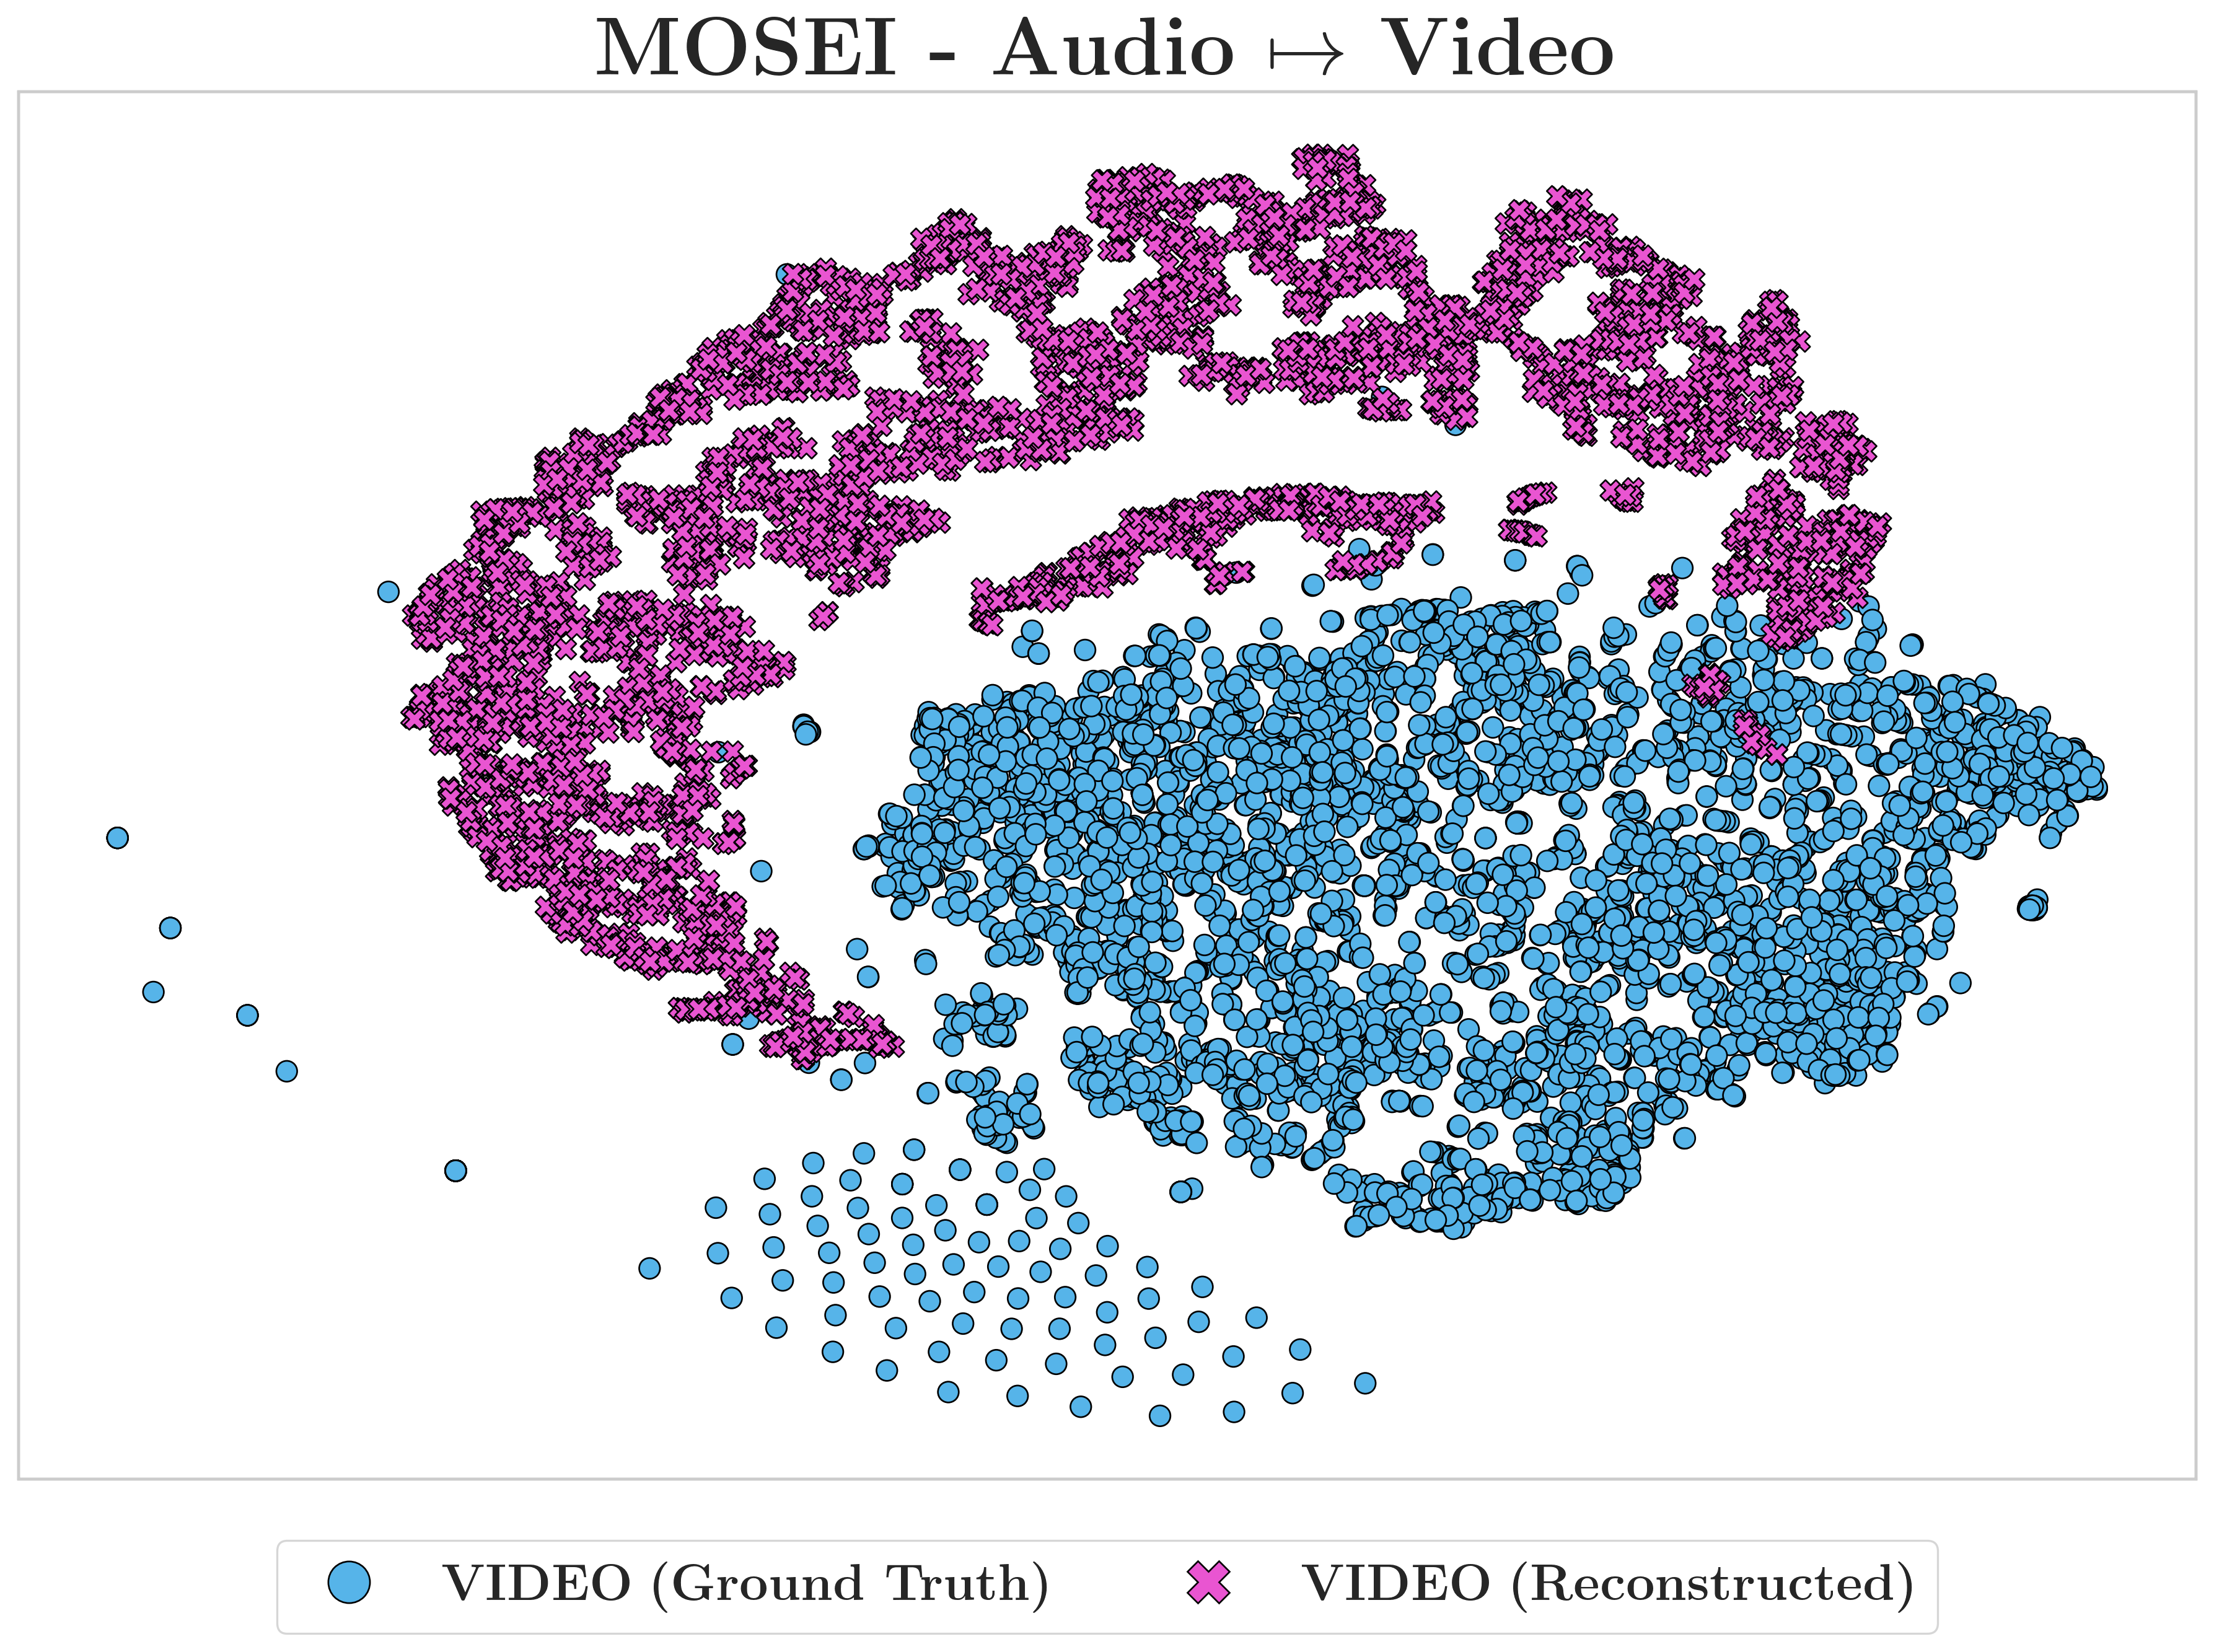
\includegraphics[width=0.33\textwidth]{imgs/MOSEI/audio_to_video/plots/tsne_embeddings_with_reconstructions.png} & 
      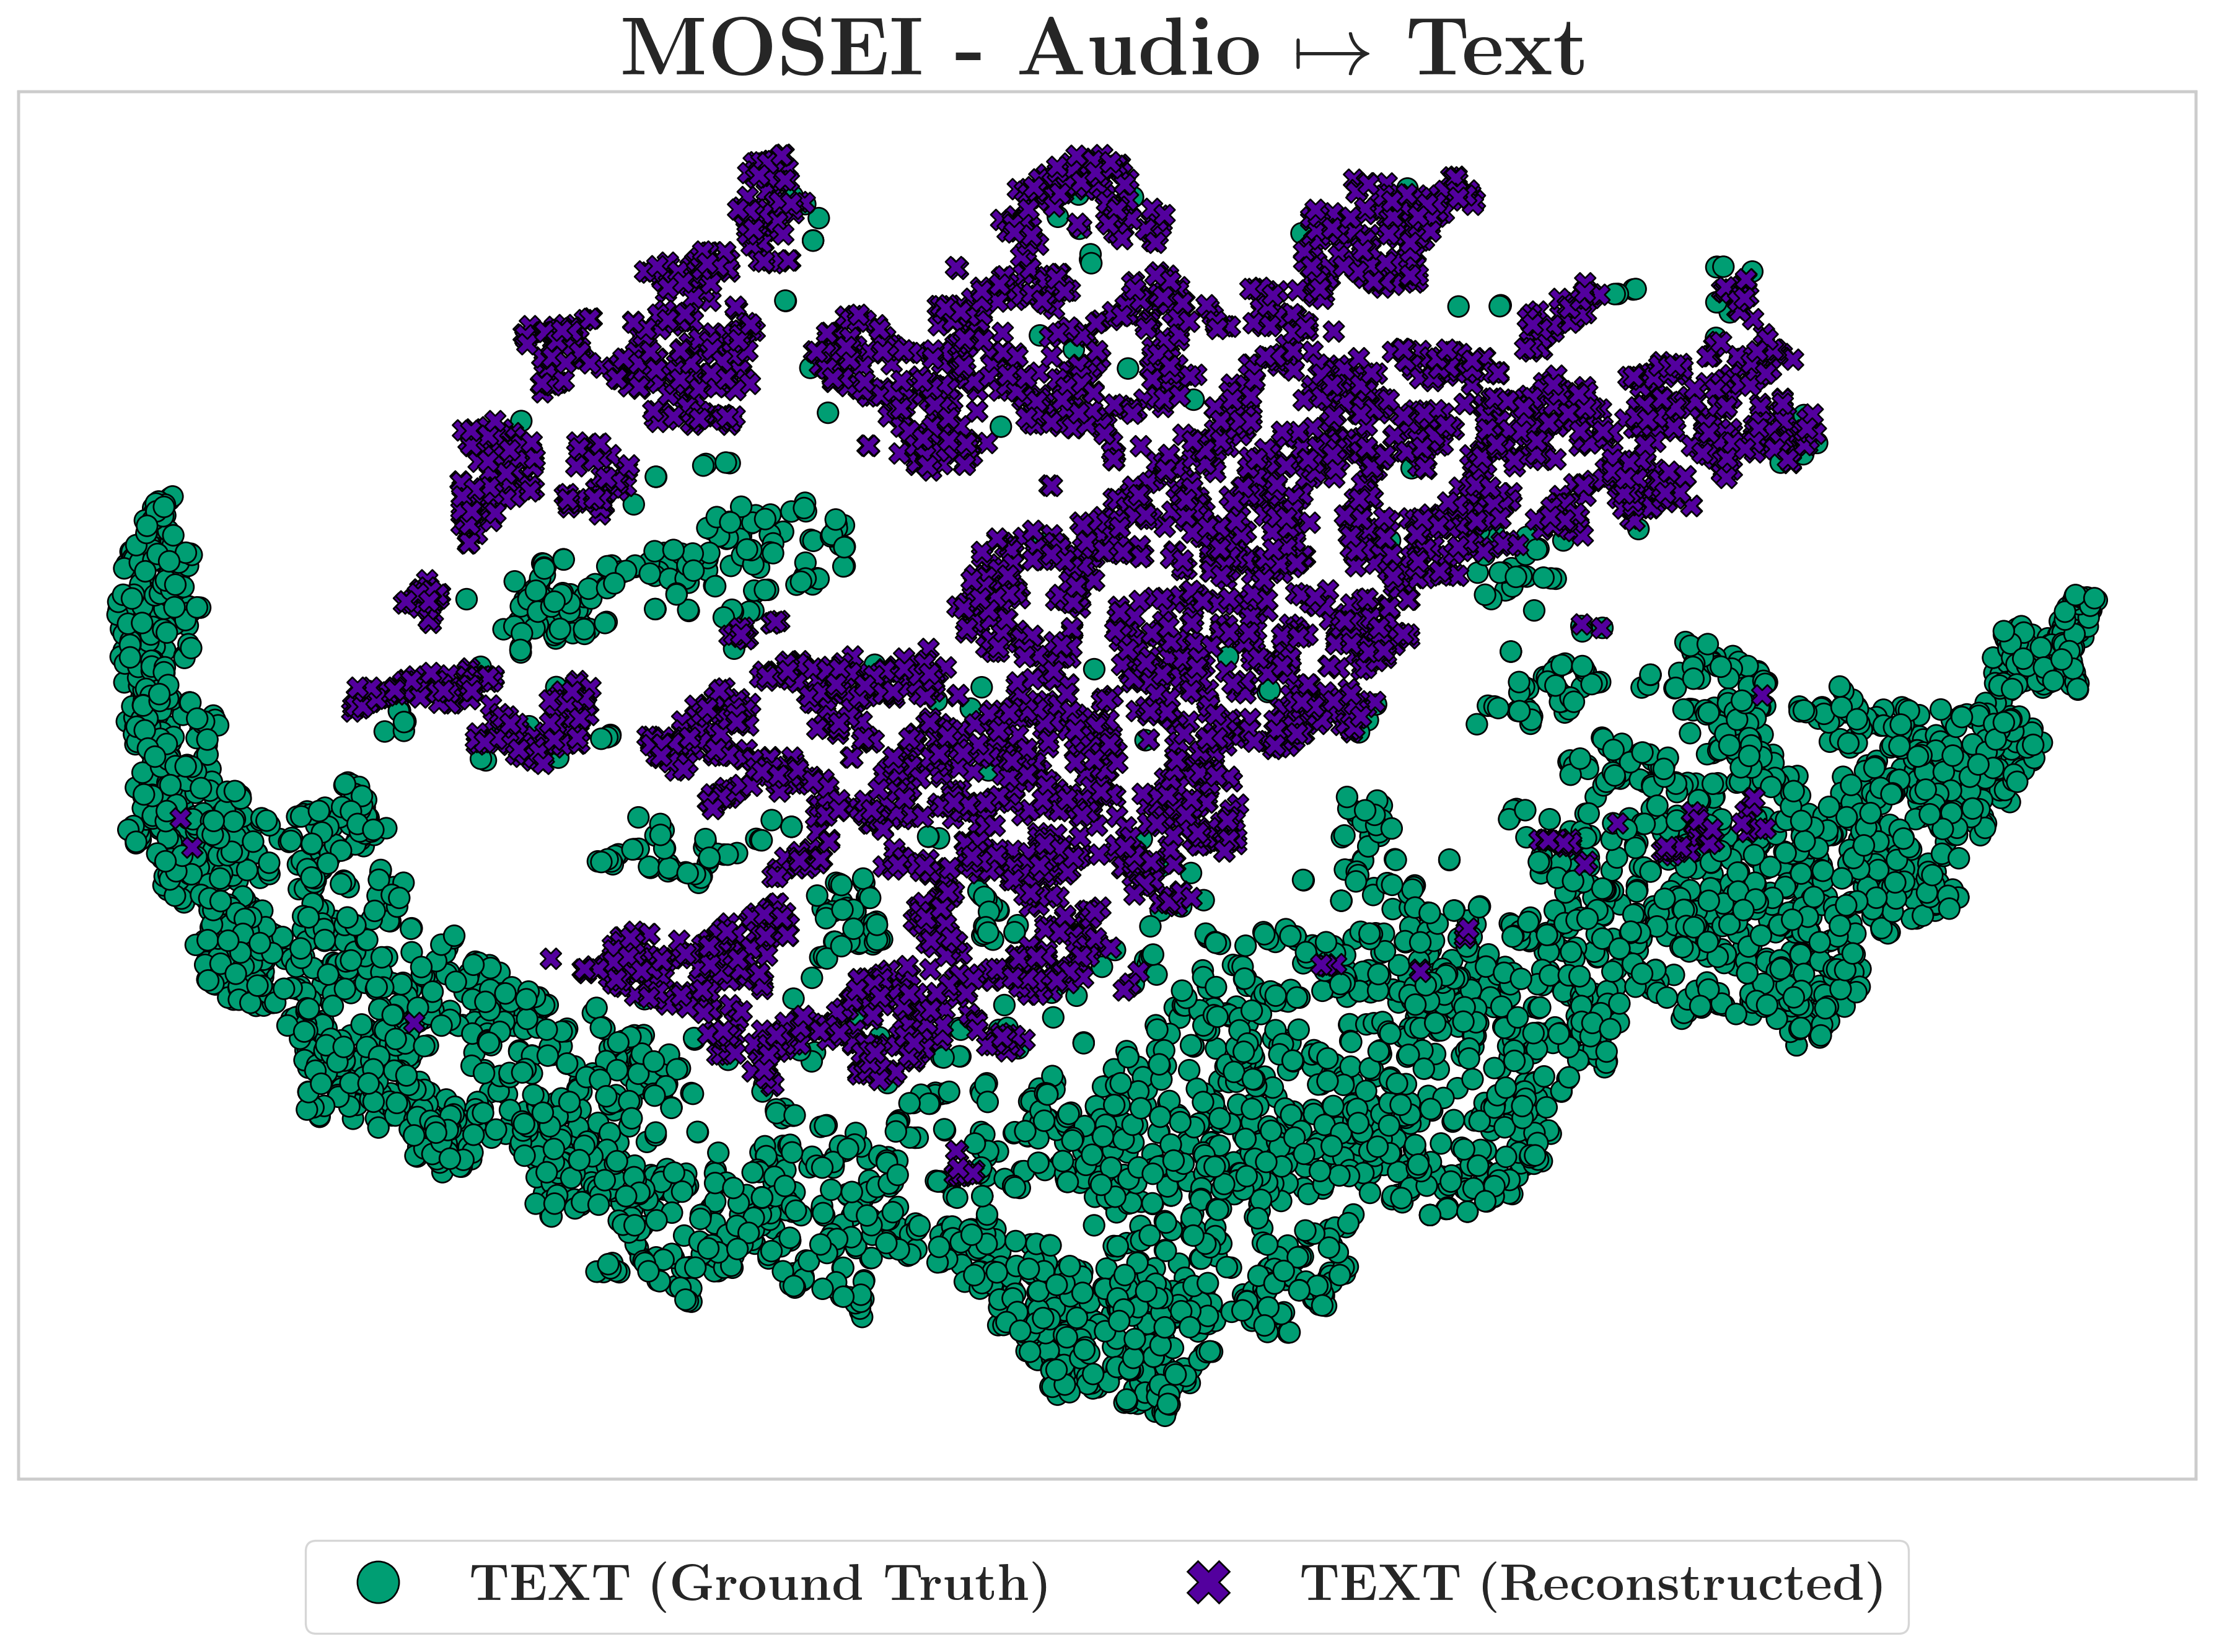
\includegraphics[width=0.33\textwidth]{imgs/MOSEI/audio_to_text/plots/tsne_embeddings_with_reconstructions.png} & 
      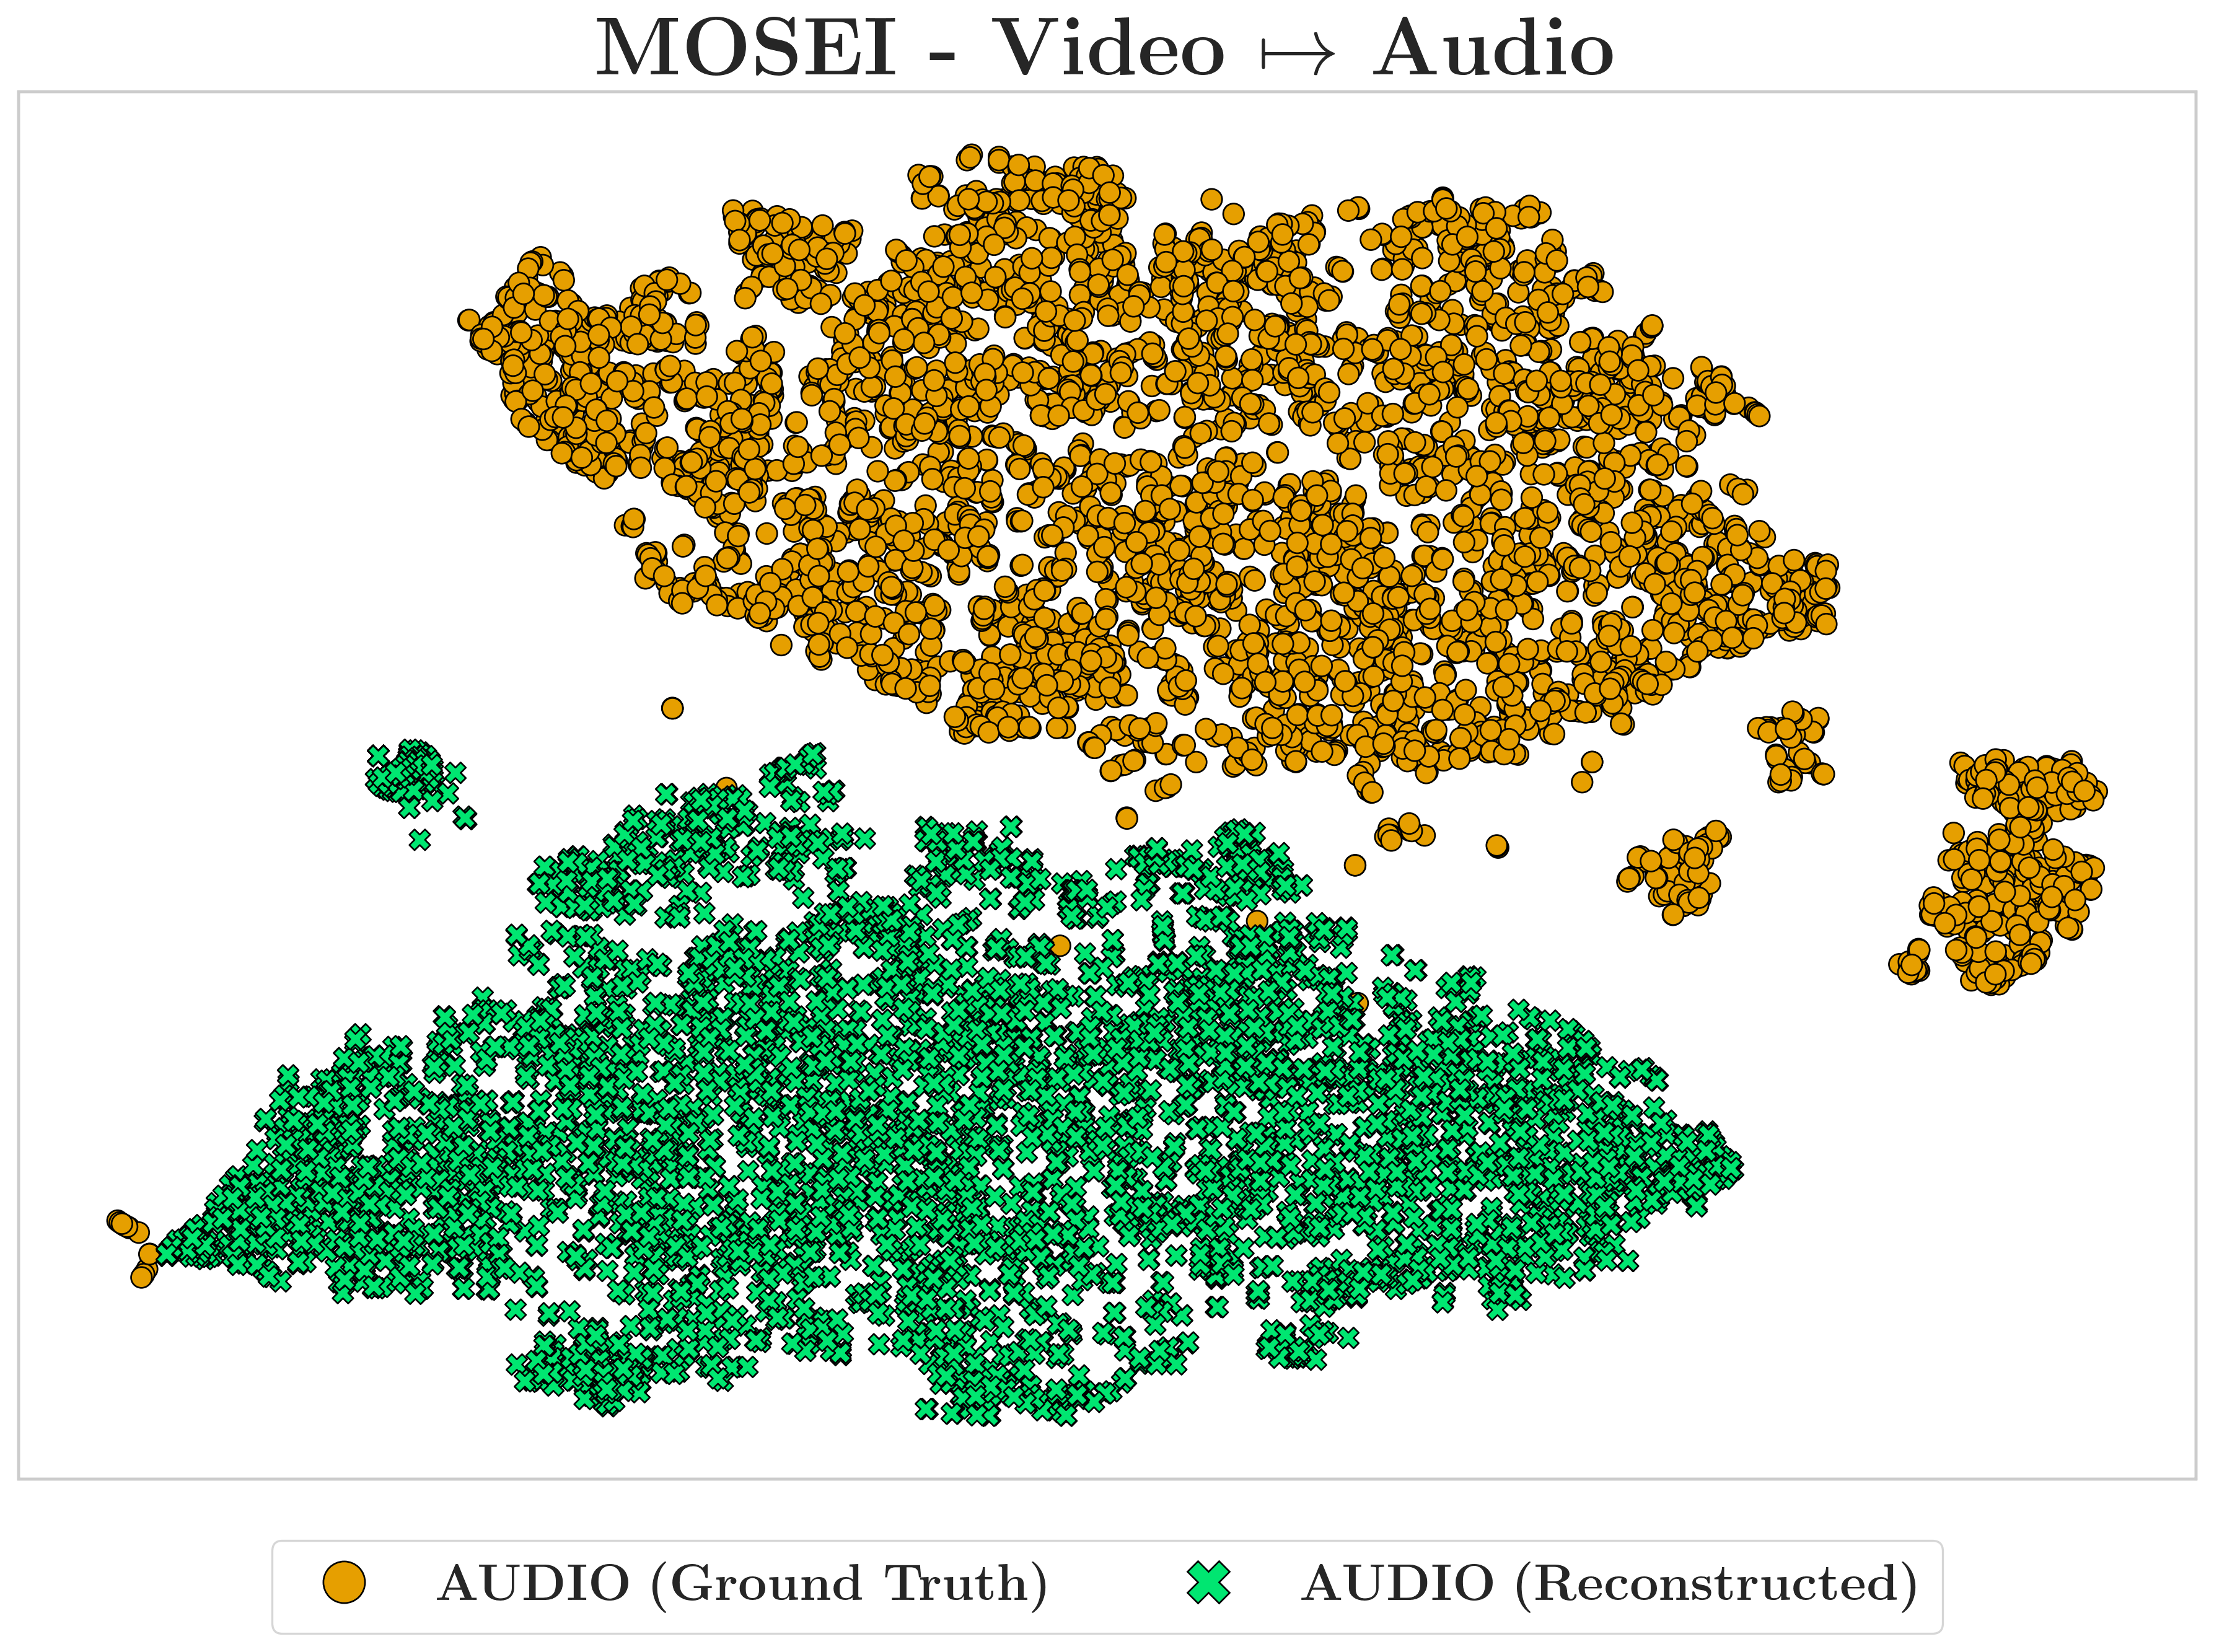
\includegraphics[width=0.33\textwidth]{imgs/MOSEI/video_to_audio/plots/tsne_embeddings_with_reconstructions.png}  \\
      
      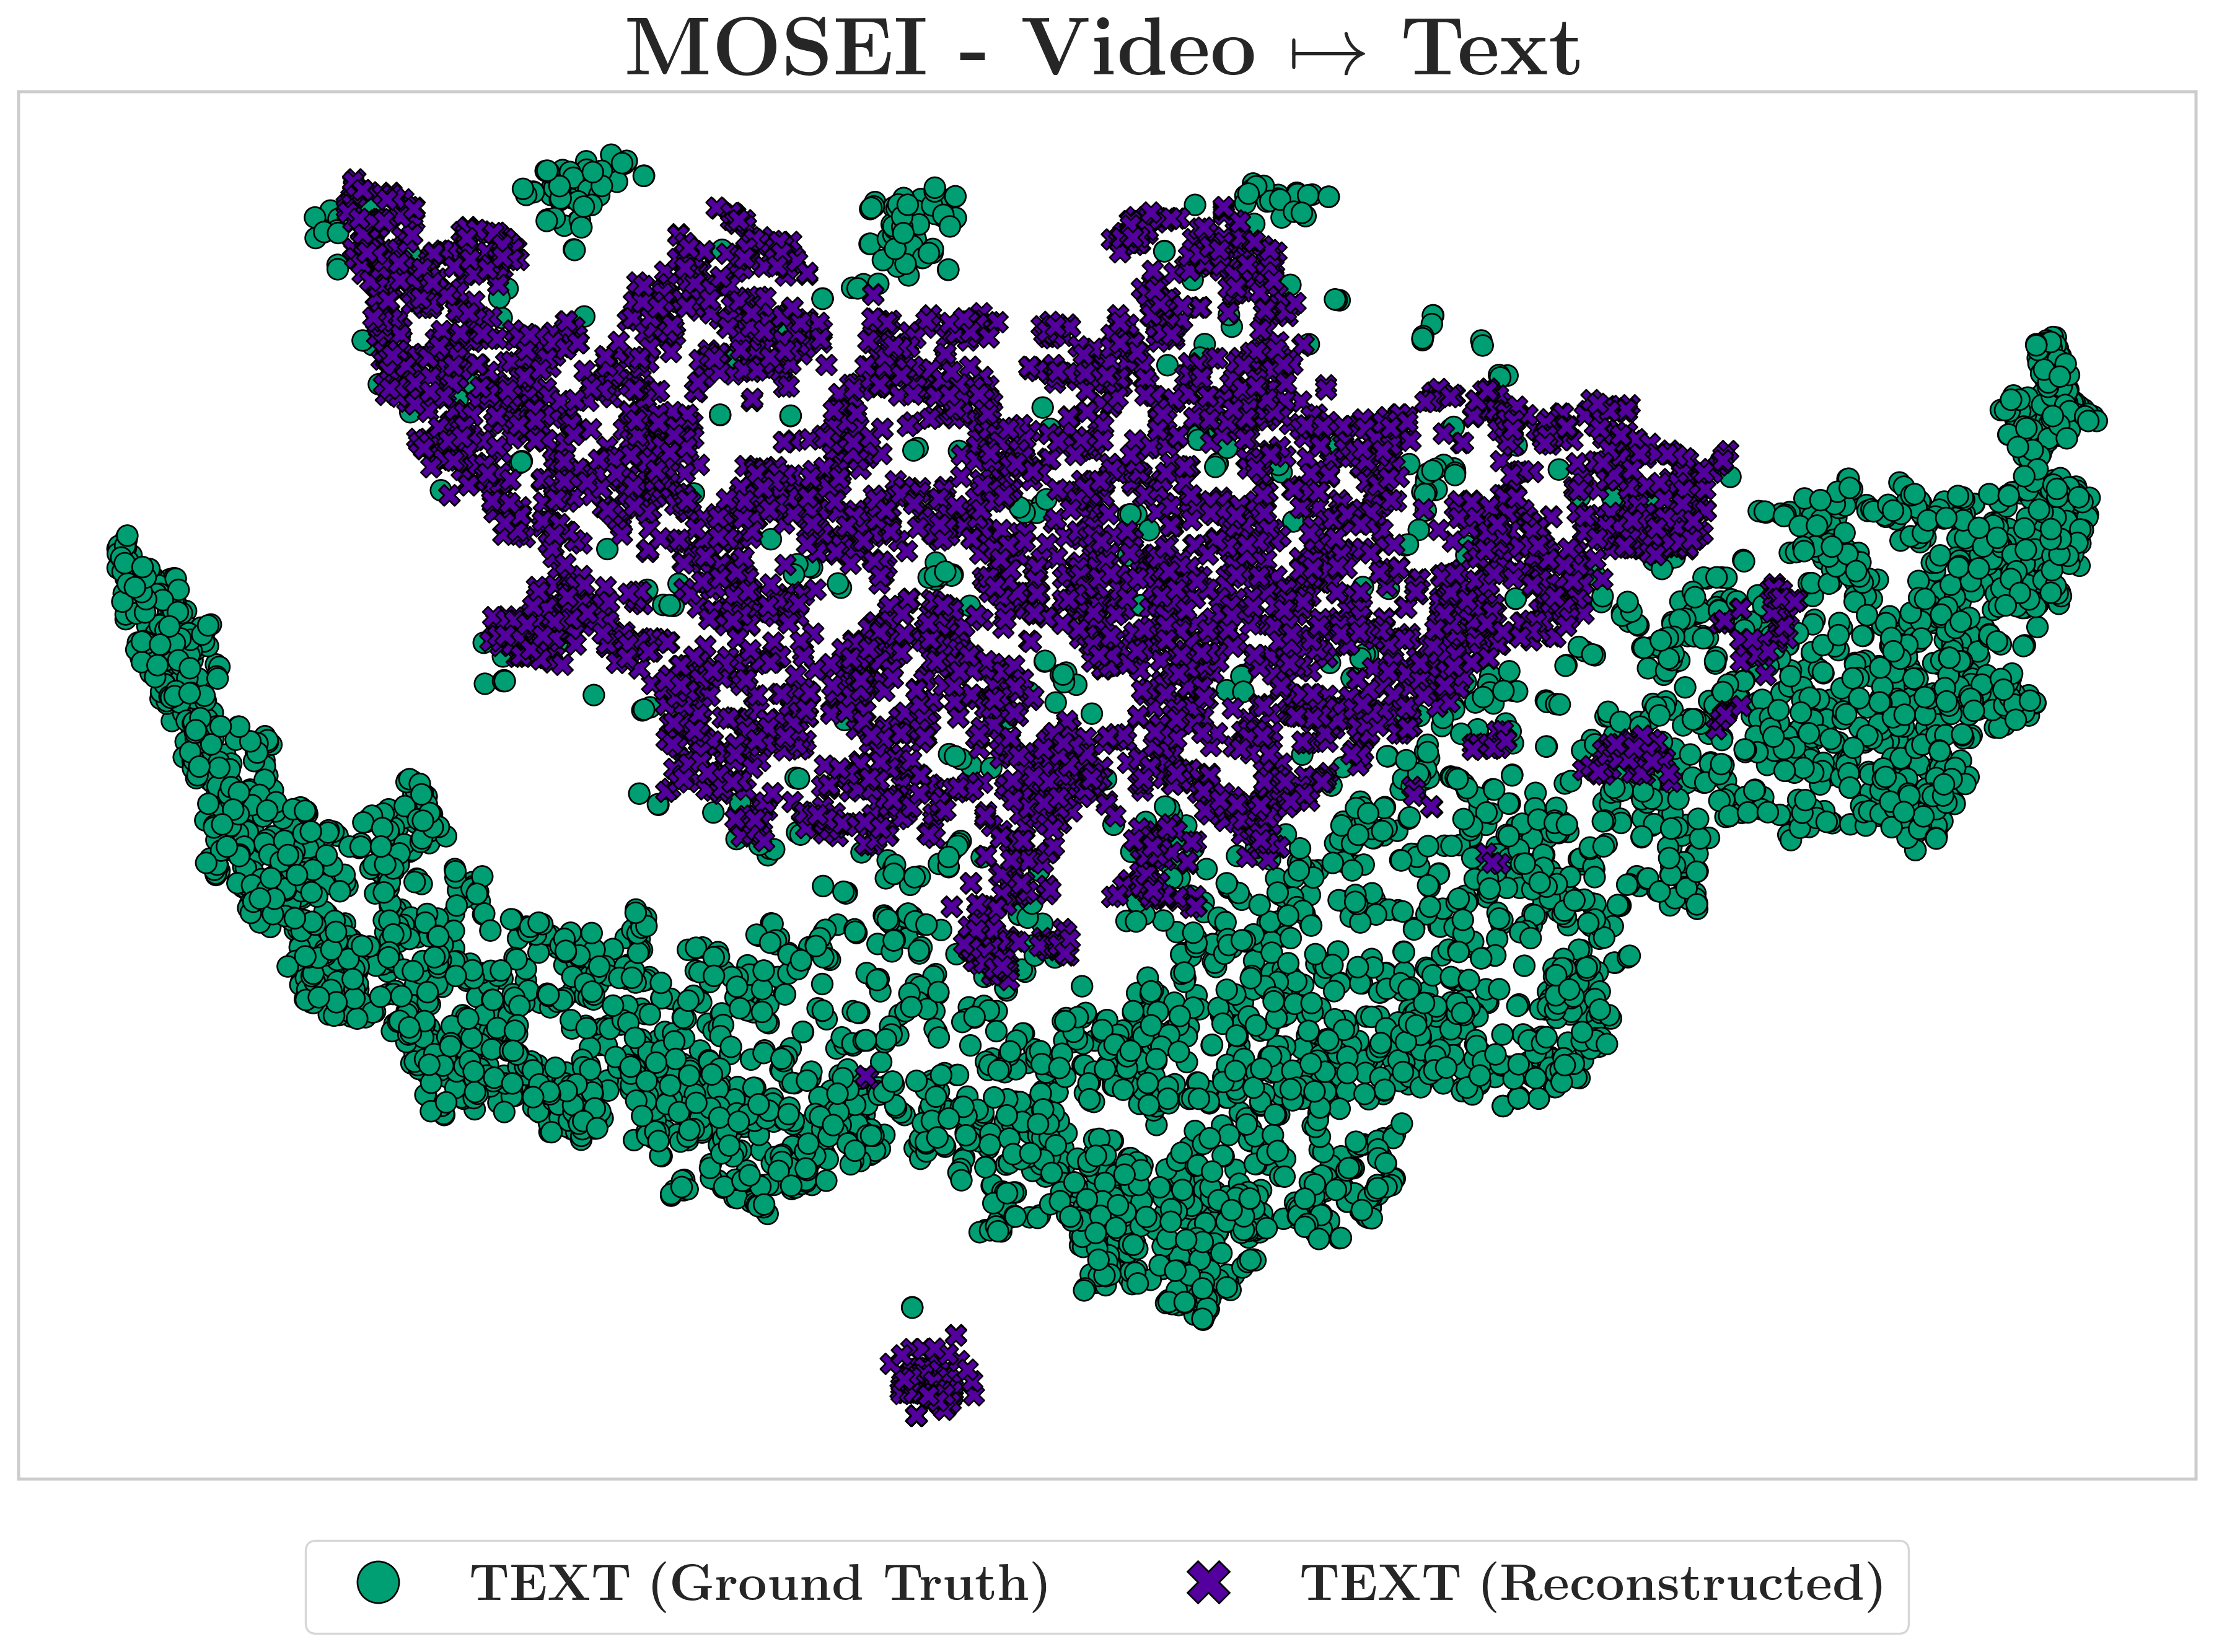
\includegraphics[width=0.33\textwidth]{imgs/MOSEI/video_to_text/plots/tsne_embeddings_with_reconstructions.png} & 
      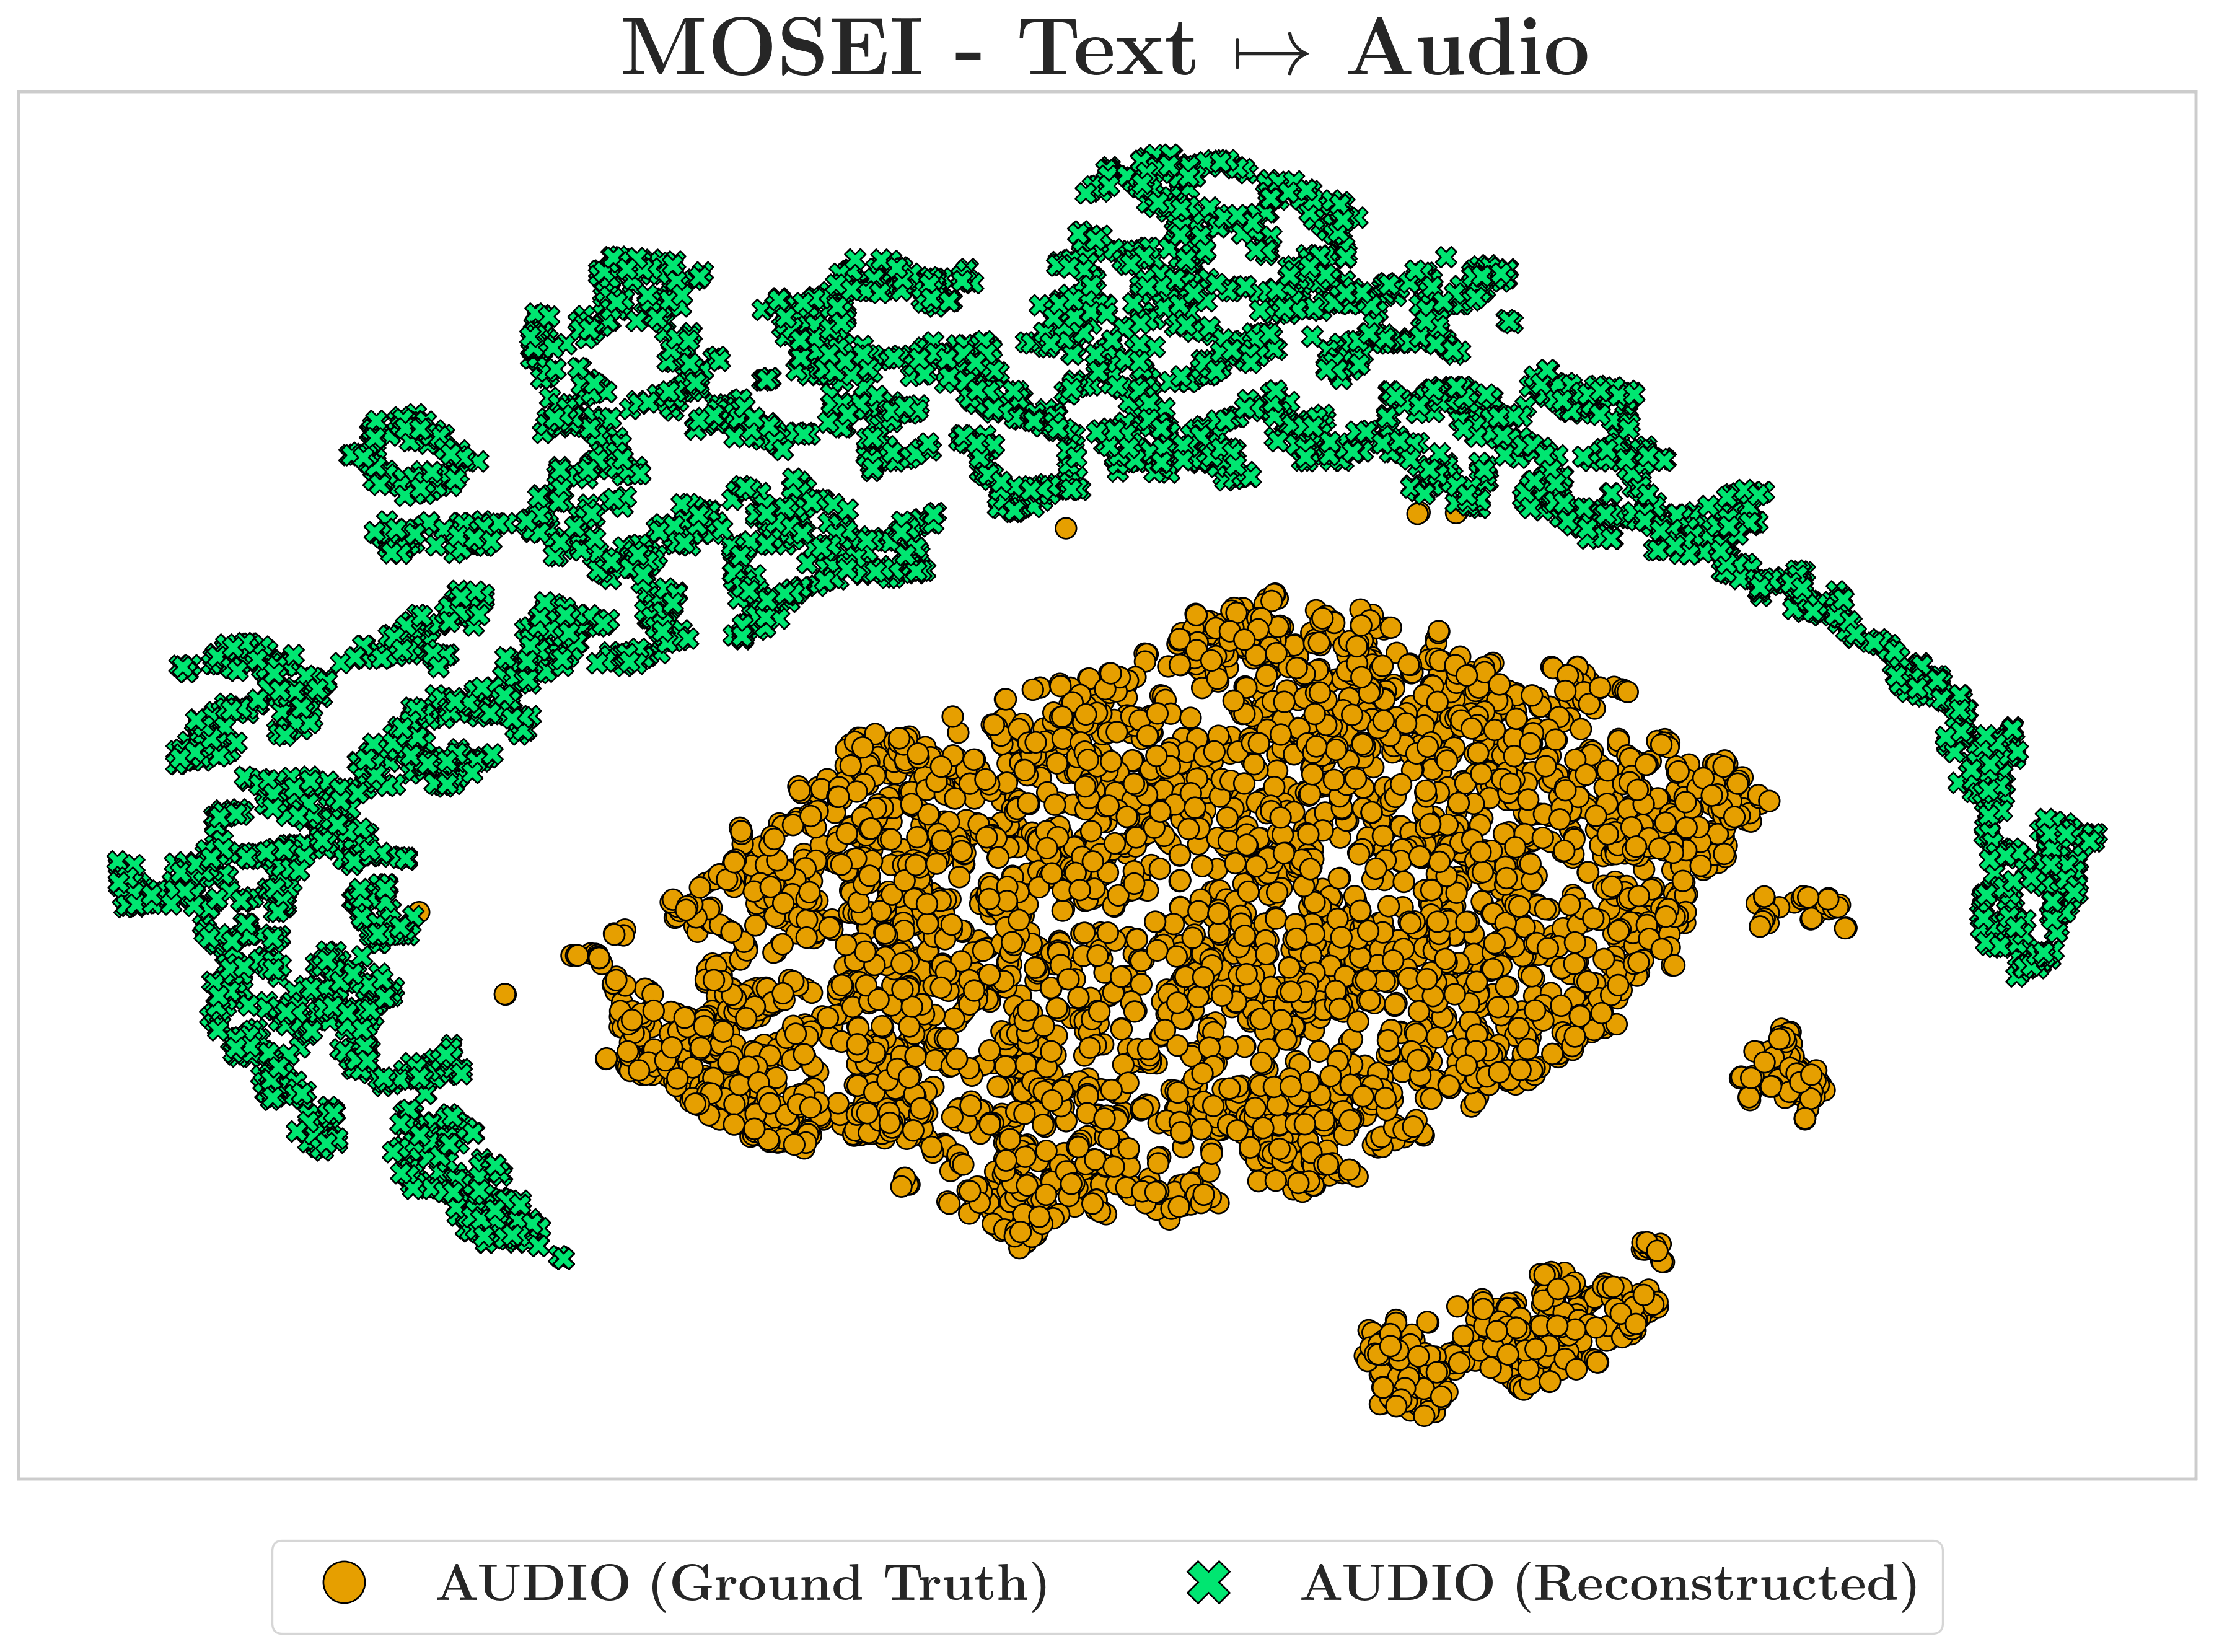
\includegraphics[width=0.33\textwidth]{imgs/MOSEI/text_to_audio/plots/tsne_embeddings_with_reconstructions.png} & 
      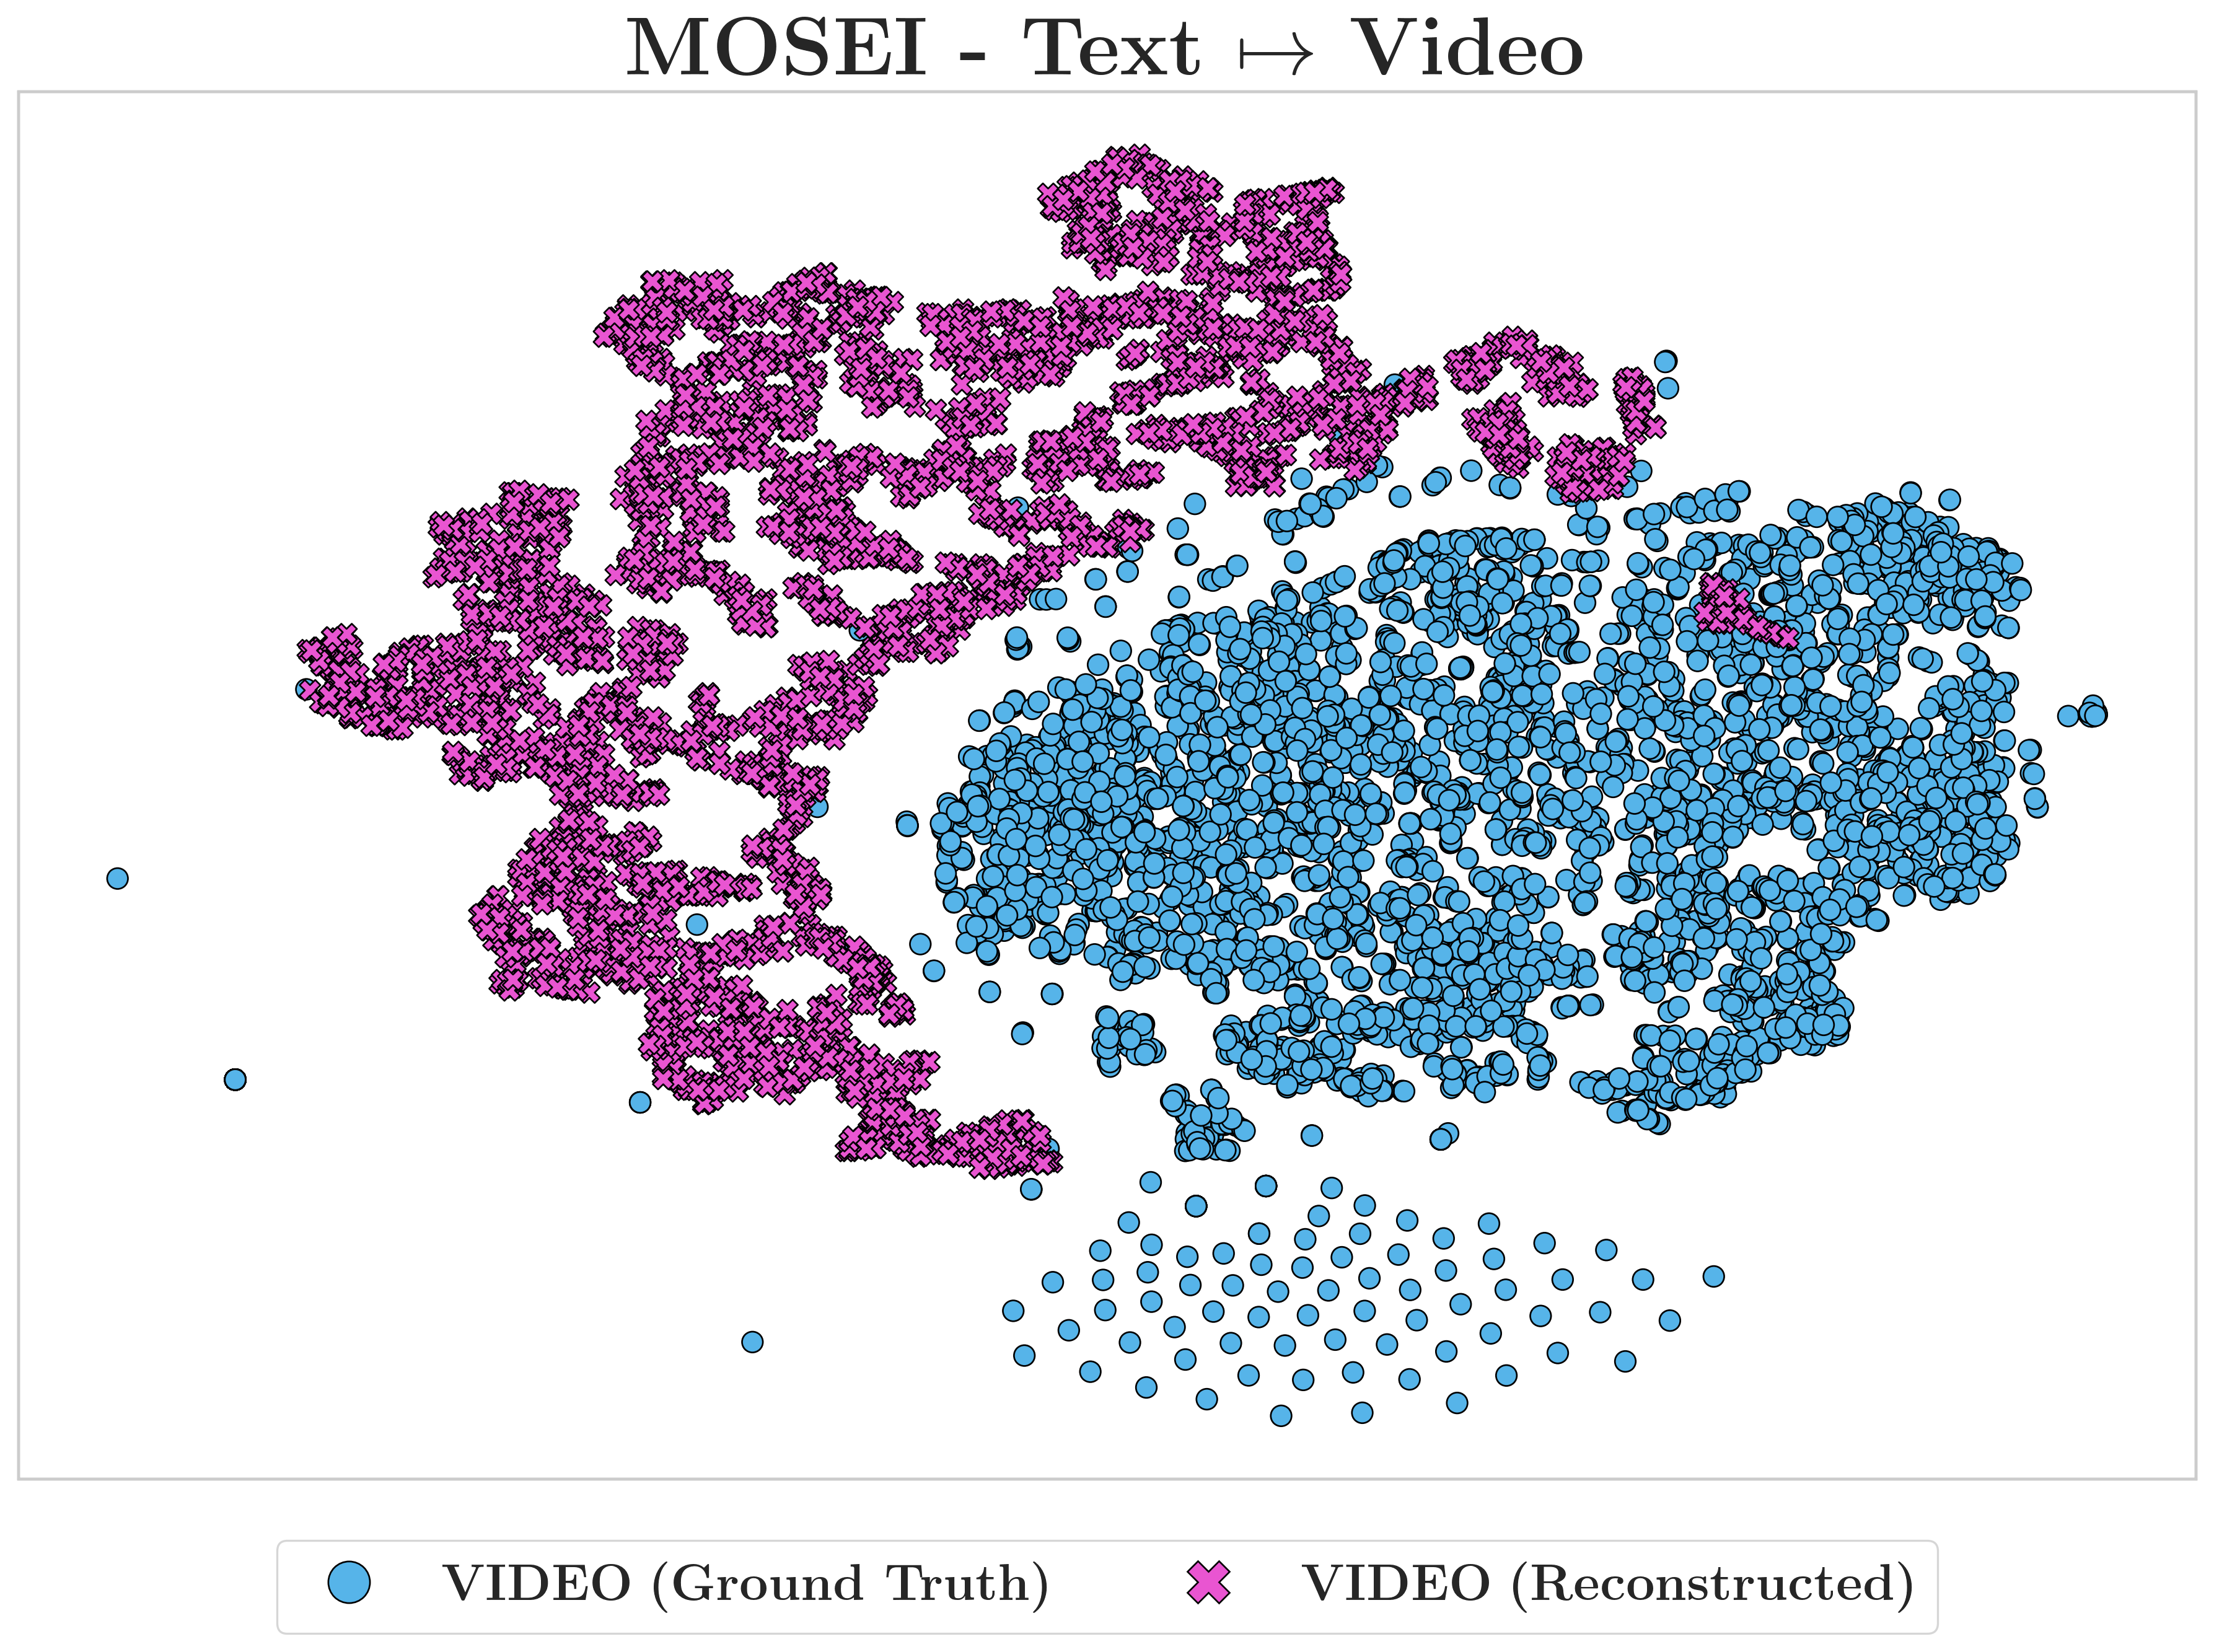
\includegraphics[width=0.33\textwidth]{imgs/MOSEI/text_to_video/plots/tsne_embeddings_with_reconstructions.png}  \\ 
      
      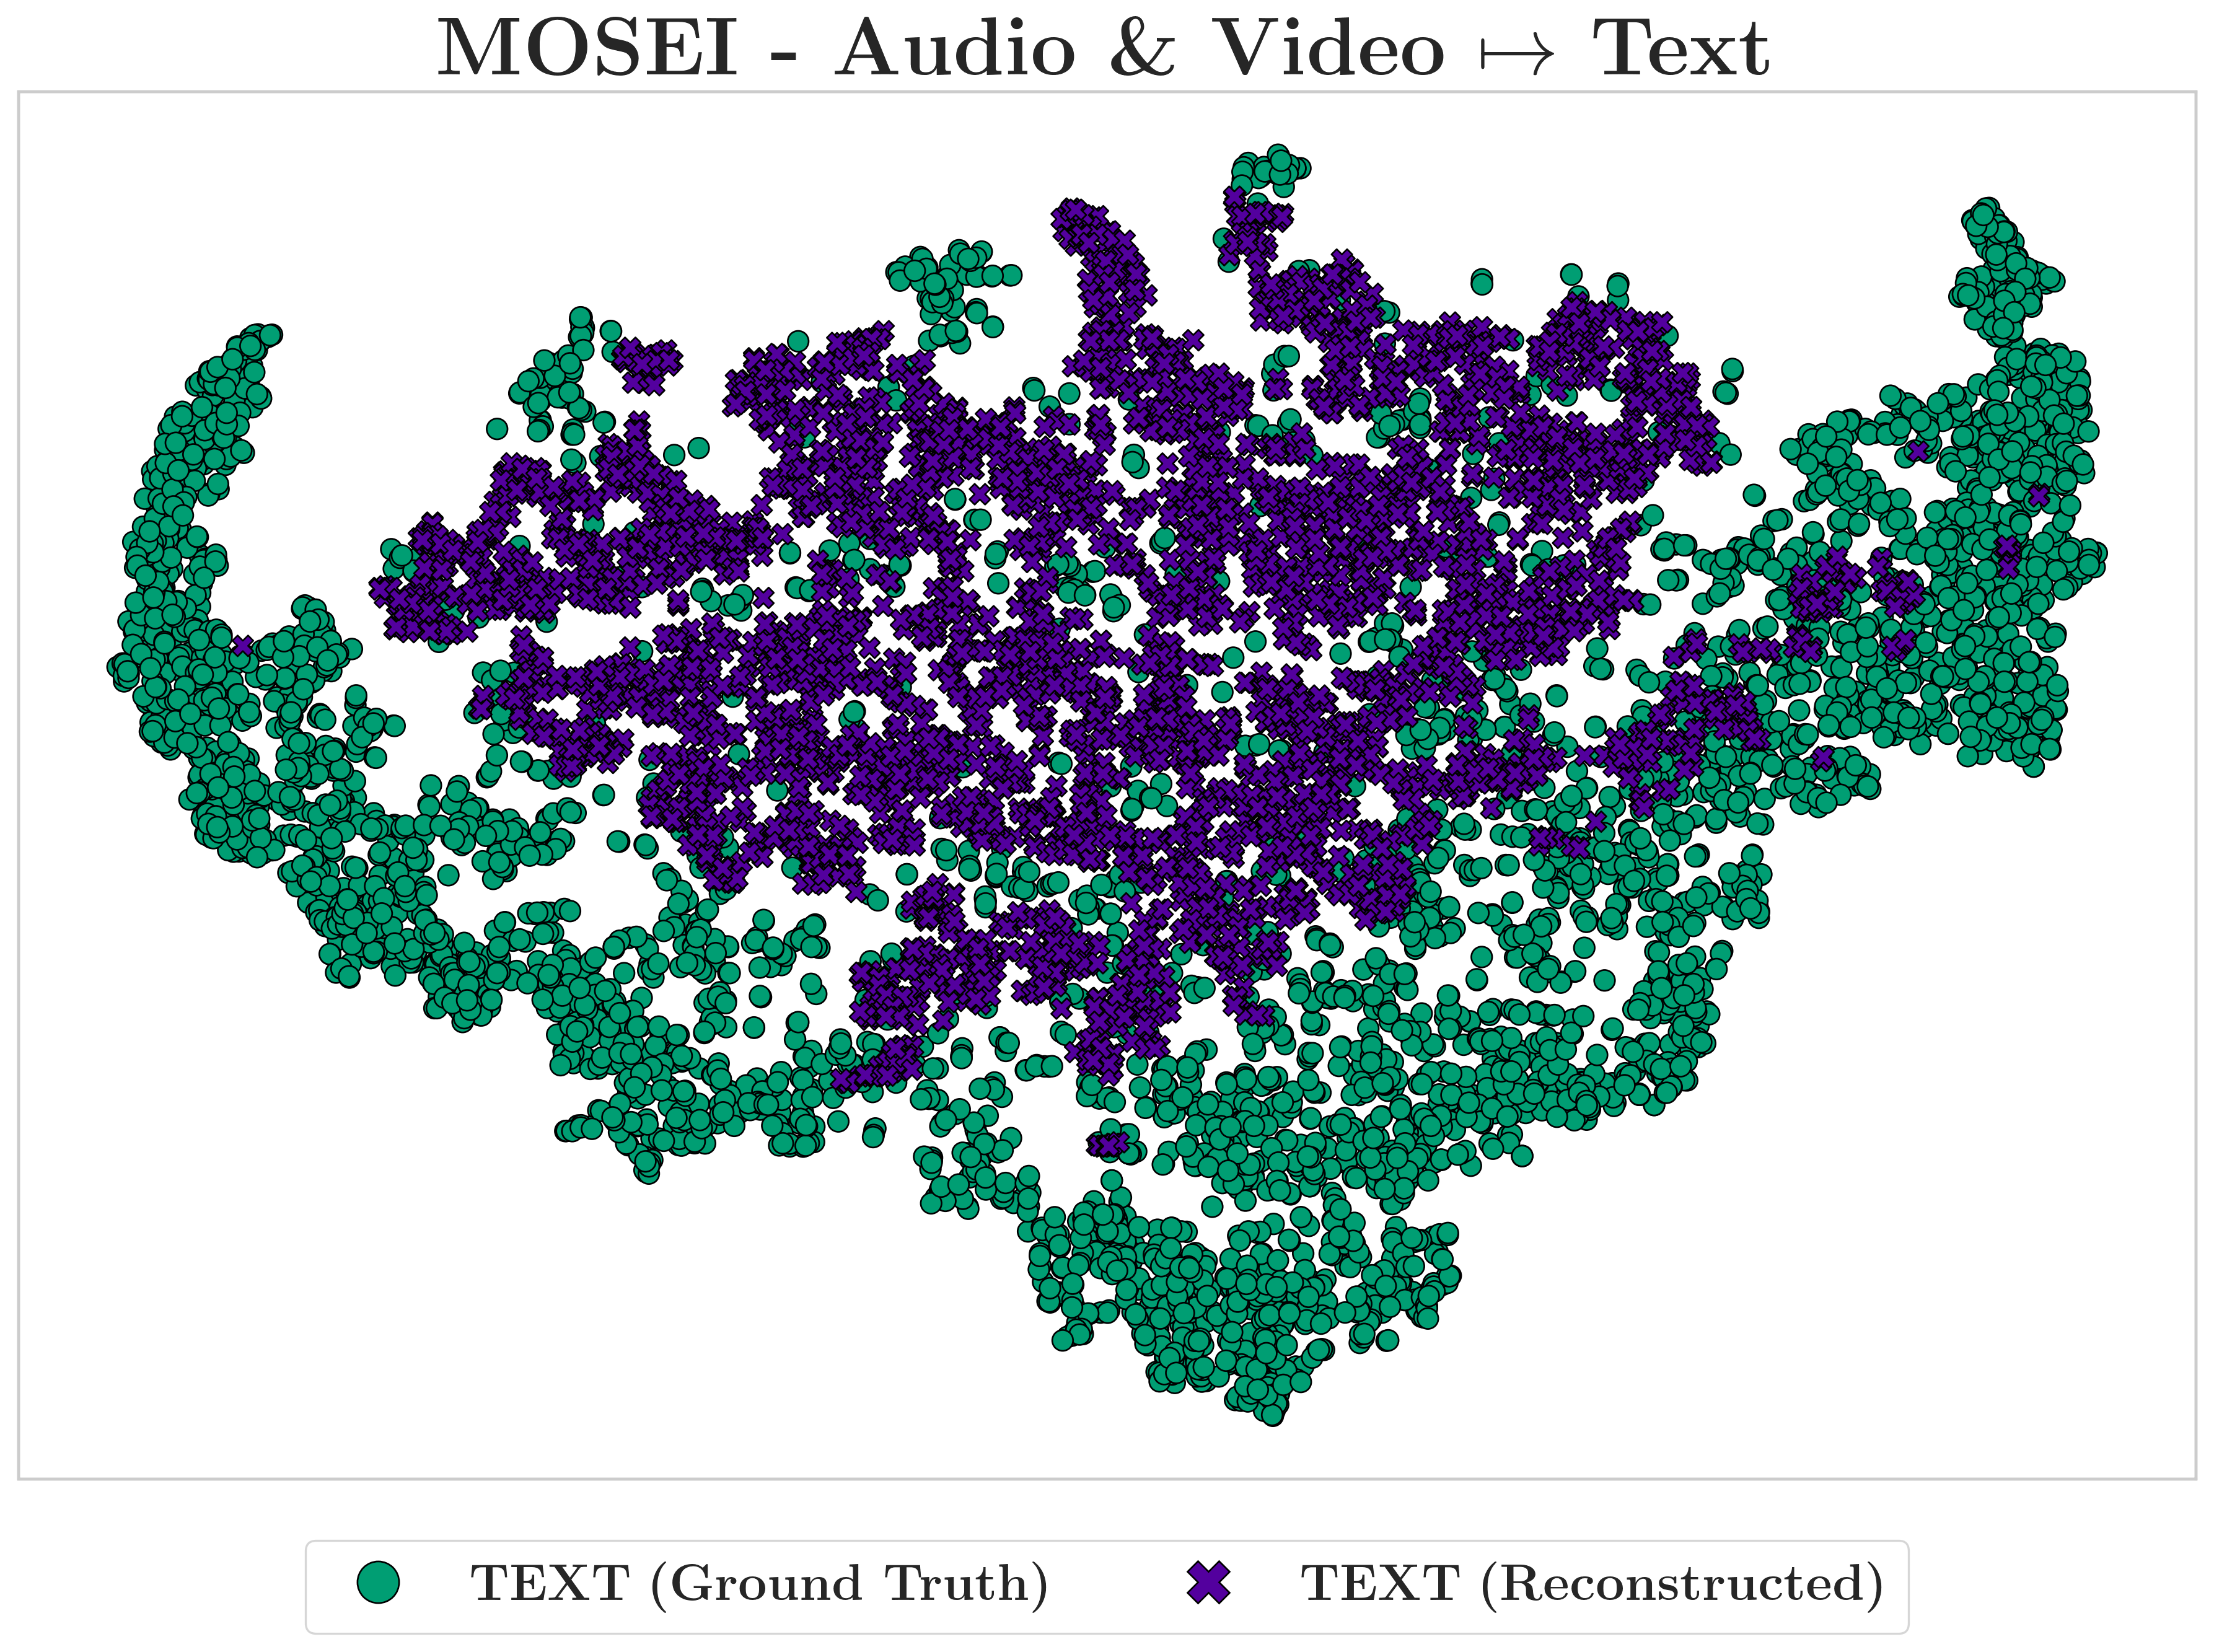
\includegraphics[width=0.33\textwidth]{imgs/MOSEI/audio_video_to_text/plots/tsne_embeddings_with_reconstructions.png} & 
      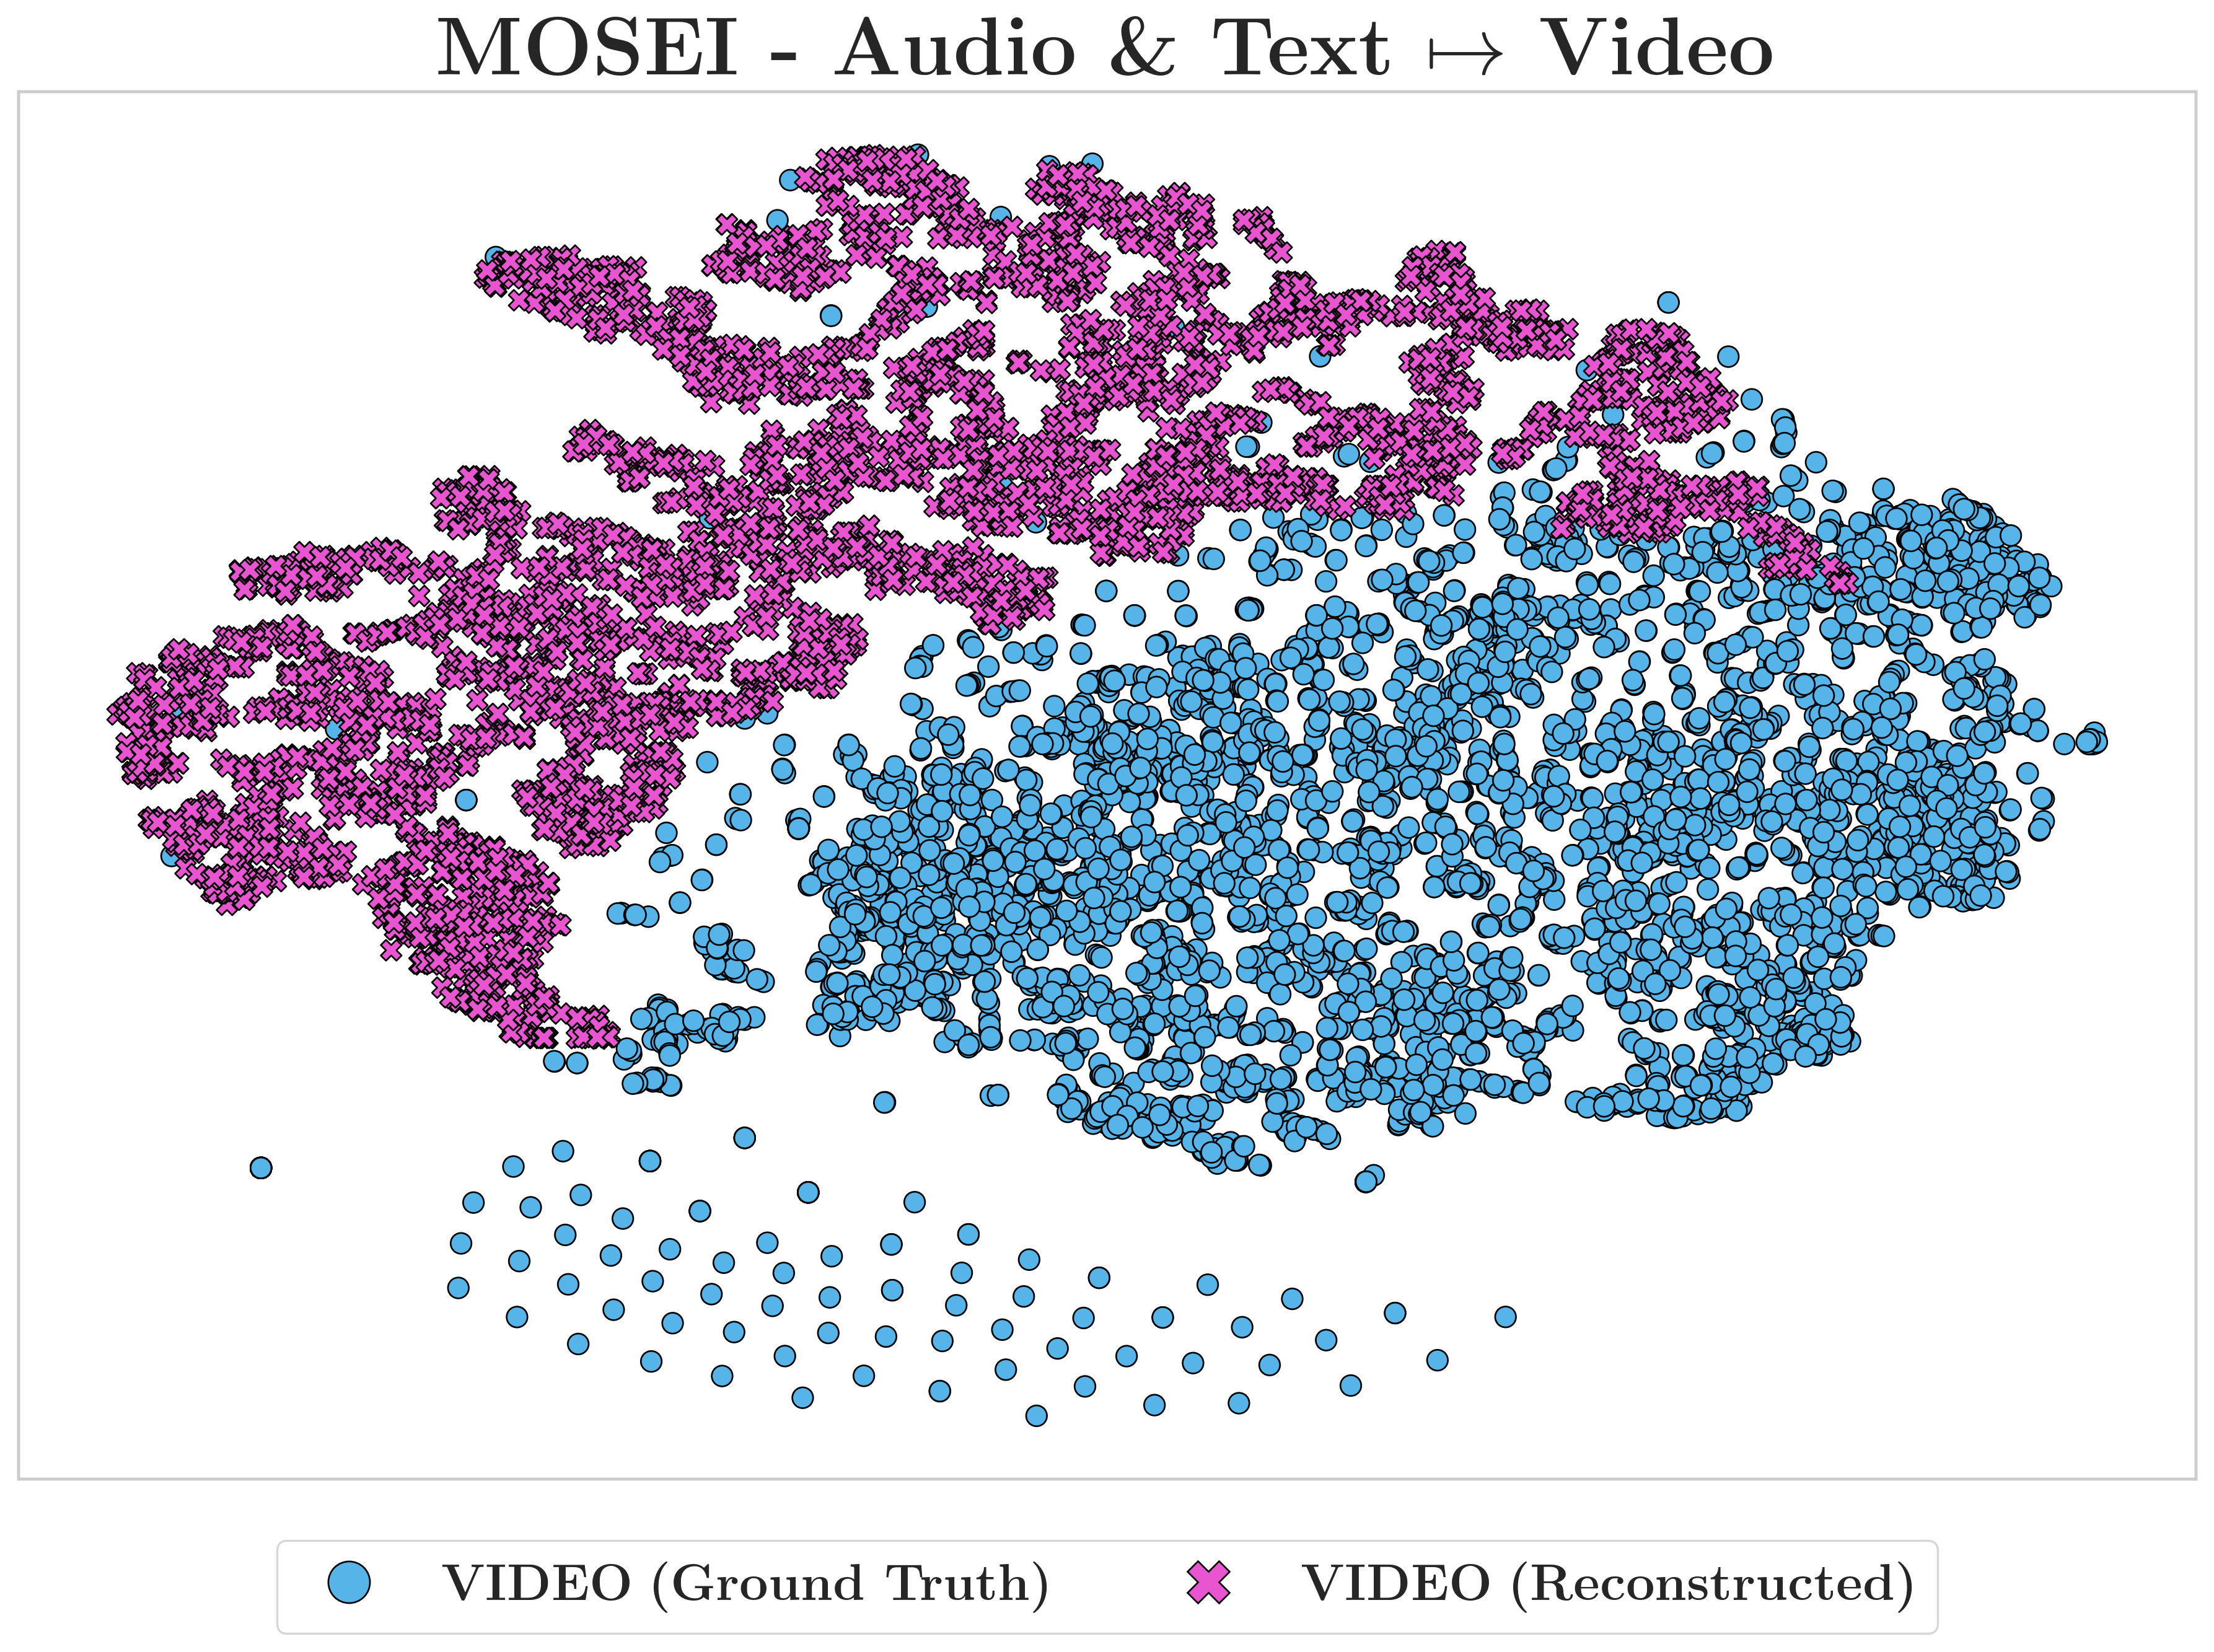
\includegraphics[width=0.33\textwidth]{imgs/MOSEI/audio_text_to_video/plots/tsne_embeddings_with_reconstructions.png}  & 
      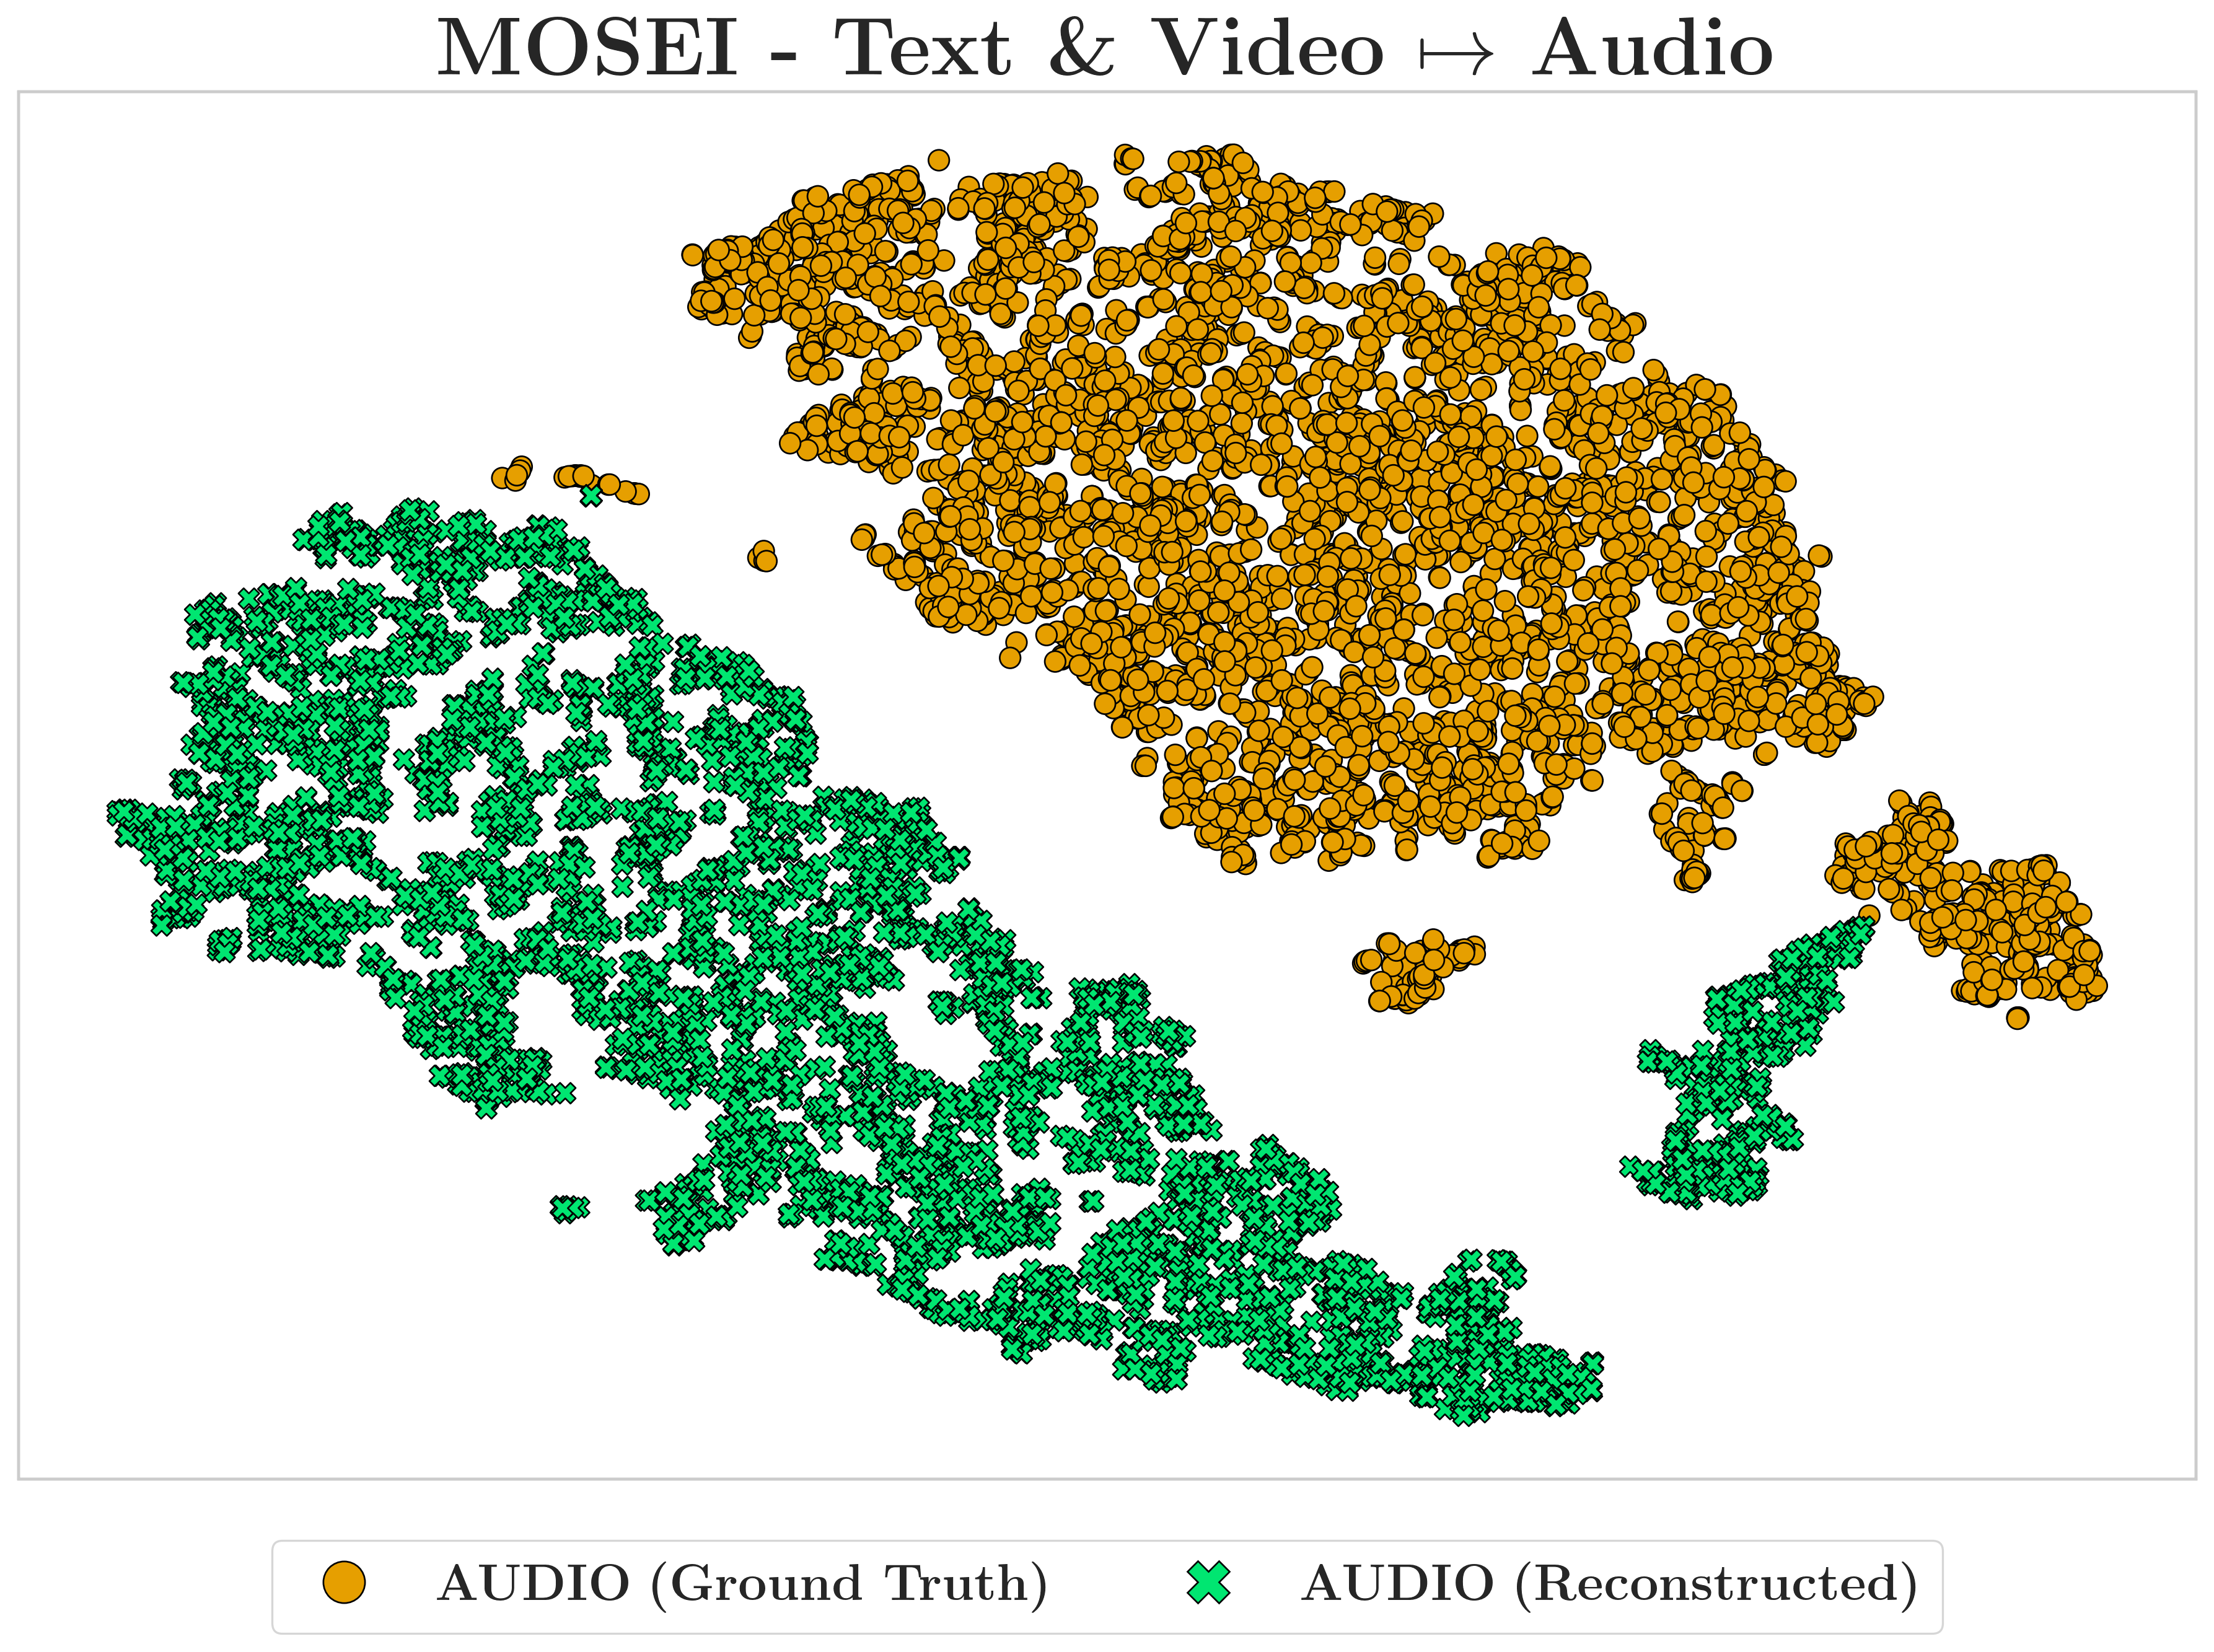
\includegraphics[width=0.33\textwidth]{imgs/MOSEI/text_video_to_audio/plots/tsne_embeddings_with_reconstructions.png} \\ 
      
    \end{tabular}
    \caption{T-SNE visualisation of the C-MAM reconstructed embeddings versus the ground truth embeddings produced by the trained modality-specific encoders for the MOSEI dataset.}
  \end{figure}


  \begin{figure}[ht!]
    \centering
    \includegraphics[width=0.99\textwidth]{imgs/MOSEI/audio_to_video/statstical_analysis.pdf}
    \includegraphics[width=0.99\textwidth]{imgs/MOSEI/audio_to_text/statstical_analysis.pdf}
    \includegraphics[width=0.99\textwidth]{imgs/MOSEI/video_to_audio/statstical_analysis.pdf}
    \end{figure}
  \begin{figure}[ht!]
    \ContinuedFloat
    \includegraphics[width=0.99\textwidth]{imgs/MOSEI/video_to_text/statstical_analysis.pdf}
    \includegraphics[width=0.99\textwidth]{imgs/MOSEI/text_to_audio/statstical_analysis.pdf}
    \includegraphics[width=0.99\textwidth]{imgs/MOSEI/text_to_video/statstical_analysis.pdf}
  \end{figure}
    \begin{figure}[ht!]
    \ContinuedFloat
    \includegraphics[width=0.99\textwidth]{imgs/MOSEI/audio_video_to_text/statstical_analysis.pdf}
    \includegraphics[width=0.99\textwidth]{imgs/MOSEI/audio_text_to_video/statstical_analysis.pdf}
    \includegraphics[width=0.99\textwidth]{imgs/MOSEI/text_video_to_audio/statstical_analysis.pdf}
    \caption{Statistical analysis of C-MAMs' reconstruction quality across the missing conditions for the MOSEI dataset. Each includes a cosine similarity distribution, dimension-wise effect size analysis, and a volcano plot for mean difference significance.}
\end{figure}

\begin{table}[hb!]
  \centering
  \caption{Reconstruction error metrics for the C-MAMs trained on the MOSEI dataset and Utterance Fusion model from \cite{zhao-etal-2021-missing}.}
  \label{tab:mosei_error_results}
  \begin{tabular}{c|cccccc}
  \hline
  \multirow{2}{*}{\textbf{Metric}} & \multicolumn{6}{c}{\textbf{MOSEI}}                                                                                                           \\ \cline{2-7} 
                                   & \textbf{A} & \textbf{V} & \textbf{T} & \textbf{AV} & \textbf{AT} & \multicolumn{1}{l}{\textbf{VT}} \\ \hline
  \textbf{MAE}                     & 0.2146           & 0.2165           & 0.1532           & 0.2135              & 0.1513              & 0.0370                                  \\
  \textbf{MSE}                     & 0.2338           & 0.2326           & 0.0415           & 0.2296              & 0.0403              & 0.0049                                  \\ \hline
  \end{tabular}%
\end{table}

\FloatBarrier

\subsection{The Role of Modality-Specific Encoders in C-MAMs}
\label{sec:encoders}
In this ablation study, we examine the impact of training modality-specific encoders within Cross-modal Association Models (C-MAMs). Specifically, we investigate whether initializing the C-MAM encoders with the weights of their corresponding modality encoders from the base multimodal model provides benefits for reconstructing missing modality embeddings, or if the association network alone is sufficient. This analysis has significant implications for training efficiency, model size, and inference performance.

To assess this, we conduct experiments using the Utterance Fusion model on the MOSEI dataset. We compare three configurations: (1) training only the association network while keeping the modality-specific encoders frozen, (2) training both the association network and encoders from randomly initialized weights, and (3) training the encoders after initializing them with their weights from the base multimodal model. The results, presented in Tables~\ref{tab:no_encoder_results} and~\ref{tab:no_encoders_mean}, highlight key trade-offs between reconstruction performance and computational cost.

\subsubsection{Performance Trade-offs}
The results demonstrate that \textbf{training encoders from scratch does not improve performance and, in many cases, degrades it} (Table~\ref{tab:no_encoders_mean}). This is particularly evident for unimodal conditions, where randomly initialised encoders perform worse than their frozen counterparts. This suggests that the association network alone is often sufficient when used in conjunction with pre-trained modality-specific embeddings.

Conversely, \textbf{initializing C-MAM encoders with their weights from the base model yields performance improvements in some cases}, particularly for \textbf{A (+0.0400) and V (+0.0451)}. However, gains are inconsistent across modalities, with negligible or negative effects observed for \textbf{T (-0.0019) and AT (-0.0050)}. These findings indicate that while weight initialisation can enhance reconstruction quality, it is not universally beneficial across all modality configurations.

\subsubsection{Computational and Storage Considerations}
A crucial consideration when training modality-specific encoders is the \textbf{increase in training time and storage requirements}. Unlike the association networks, which are inherently lightweight in this work, incorporating additional encoders would significantly increase the overall model size and computational cost. Table~\ref{tab:param_counts} provides resource measurements for the association model alone, illustrating its efficiency. Since training encoders introduces additional parameters and storage overhead, their inclusion would result in a model that is substantially larger and computationally more demanding compared to using the association network alone. Training just the association network also leads to decreased inference times as the embeddings produced by the base model are used for both classification and reconstruction, whereas if the C-MAM encoders are trained in any way, then they must be used at inference time, increasing the time taken to make a prediction.

\subsubsection{Flexible Training Strategies}
A key advantage of the C-MAM framework is its \textbf{flexibility in training strategies}. Since reconstruction is fully decoupled from the classification task, different configurations can be tailored to specific requirements. For example, in practical deployments, one could \textbf{train C-MAM encoders using their initialized weights only for critical modalities while training the remaining association models without them}. This selective training approach enables a balance between performance and efficiency, ensuring that C-MAMs can be adapted to varying computational constraints.

\subsubsection{Conclusion}
These results indicate that \textbf{the association network alone is often sufficient}, with C-MAM encoders initialized with their weights from the base multimodal model offering improvements only in select cases. Moreover, while training these encoders can enhance reconstruction quality, it comes at the cost of increased training time and storage requirements. The modular nature of C-MAMs enables \textbf{task-specific optimization}, allowing practitioners to selectively train encoders based on the demands of the application. Future work will extend this analysis to more models and datasets. 



\begin{table}[]
\centering
\caption{Performance comparison between training the association model only, training the association model with the modality-specific encoders from randomly initialised weights (from scratch) and training the association model with the modality-specific encoders initialised with the weight of the corresponding encoder in the base multimodal model. }
\label{tab:no_encoder_results}
\resizebox{\textwidth}{!}{%
\begin{tabular}{cl|ccccc}
\hline
\textbf{\begin{tabular}[c]{@{}c@{}}Modalities\\ Available\end{tabular}} &
  \multicolumn{1}{c|}{\textbf{Metric}} &
  \textbf{\begin{tabular}[c]{@{}c@{}}Association\\ Only\end{tabular}} &
  \textbf{\begin{tabular}[c]{@{}c@{}}Randomly \\ Initialised Encoders\end{tabular}} &
  \textbf{\begin{tabular}[c]{@{}c@{}}Random \\ Initialisation Difference\end{tabular}} &
  \textbf{\begin{tabular}[c]{@{}c@{}}Fine-tuned\\ Encoders\end{tabular}} &
  \textbf{\begin{tabular}[c]{@{}c@{}}Fine-tuned \\ Difference\end{tabular}} \\ \hline
\multirow{4}{*}{\textbf{A}}  & \textbf{Non0 Accuracy}    & 0.5802 & 0.5808 & \textbf{0.0006}  & 0.6265 & \textbf{0.0463} \\
                             & \textbf{Has0 Accuracy}    & 0.6154 & 0.5754 & \textbf{-0.0400} & 0.6613 & \textbf{0.0459} \\
                             & \textbf{Non0 F1 Weighted} & 0.5809 & 0.5665 & \textbf{-0.0144} & 0.6201 & \textbf{0.0392} \\
                             & \textbf{Has0 F1 Weighted} & 0.6357 & 0.5814 & \textbf{-0.0543} & 0.6641 & \textbf{0.0284} \\ \hline
\multirow{4}{*}{\textbf{V}}  & \textbf{Non0 Accuracy}    & 0.6036 & 0.6179 & \textbf{0.0143}  & 0.6214 & \textbf{0.0178} \\
                             & \textbf{Has0 Accuracy}    & 0.6779 & 0.6844 & \textbf{0.0065}  & 0.7421 & \textbf{0.0642} \\
                             & \textbf{Non0 F1 Weighted} & 0.5739 & 0.5908 & \textbf{0.0169}  & 0.6178 & \textbf{0.0439} \\
                             & \textbf{Has0 F1 Weighted} & 0.6492 & 0.6539 & \textbf{0.0047}  & 0.7037 & \textbf{0.0545} \\ \hline
\multirow{4}{*}{\textbf{T}}  & \textbf{Non0 Accuracy}    & 0.8181 & 0.8035 & -0.0146          & 0.8139 & -0.0042         \\
                             & \textbf{Has0 Accuracy}    & 0.7690 & 0.7496 & -0.0194          & 0.7678 & -0.0012         \\
                             & \textbf{Non0 F1 Weighted} & 0.8202 & 0.8056 & -0.0146          & 0.8162 & -0.0040         \\
                             & \textbf{Has0 F1 Weighted} & 0.7482 & 0.7401 & -0.0081          & 0.7502 & 0.0020          \\ \hline
\multirow{4}{*}{\textbf{AV}} & \textbf{Non0 Accuracy}    & 0.6279 & 0.6504 & 0.0225           & 0.6439 & 0.0160          \\
                             & \textbf{Has0 Accuracy}    & 0.7434 & 0.7419 & -0.0015          & 0.7345 & -0.0089         \\
                             & \textbf{Non0 F1 Weighted} & 0.6241 & 0.6468 & 0.0227           & 0.6434 & 0.0193          \\
                             & \textbf{Has0 F1 Weighted} & 0.7026 & 0.7008 & -0.0018          & 0.6999 & -0.0027         \\ \hline
\multirow{4}{*}{\textbf{AT}} & \textbf{Non0 Accuracy}    & 0.8154 & 0.8059 & -0.0095          & 0.8075 & -0.0079         \\
                             & \textbf{Has0 Accuracy}    & 0.7665 & 0.7621 & -0.0044          & 0.7648 & -0.0017         \\
                             & \textbf{Non0 F1 Weighted} & 0.8181 & 0.8087 & -0.0094          & 0.8102 & -0.0079         \\
                             & \textbf{Has0 F1 Weighted} & 0.7550 & 0.7516 & -0.0034          & 0.7526 & -0.0024         \\ \hline
\multirow{4}{*}{\textbf{VT}} & \textbf{Non0 Accuracy}    & 0.8095 & 0.8149 & \textbf{0.0054}  & 0.8123 & \textbf{0.0028} \\
                             & \textbf{Has0 Accuracy}    & 0.7633 & 0.7668 & \textbf{0.0035}  & 0.7644 & \textbf{0.0011} \\
                             & \textbf{Non0 F1 Weighted} & 0.8122 & 0.8173 & \textbf{0.0051}  & 0.8149 & \textbf{0.0027} \\
                             & \textbf{Has0 F1 Weighted} & 0.7508 & 0.7550 & \textbf{0.0042}  & 0.7510 & \textbf{0.0002} \\ \hline
\end{tabular}%
}
\end{table}

\begin{table}[]
\centering
\caption{Mean difference in performance (relative to not training just the association network) across four metrics, Has0 Accuracy, Non0 Accuracy, Has0 F1-Weighted, and Non0 F1-Weighted, when including modality-specific encoders for six different modality conditions. The “Encoders From Scratch” column shows the performance change when training new encoders from randomly initialized weights, whereas “Encoders Fine-tuned” shows the performance change when starting from pre-trained encoders of the base multimodal model and then further training them for modality reconstruction. Negative values indicate lower performance compared to the baseline (no encoder training), and positive values indicate performance improvements.}
\label{tab:no_encoders_mean}
\begin{tabular}{c|cc}
\hline
 & \textbf{\begin{tabular}[c]{@{}c@{}}Randomly\\ Initialised Encoders\end{tabular}} & \textbf{\begin{tabular}[c]{@{}c@{}}Fine-tuned\\ Encoders\end{tabular}} \\ \hline
\textbf{A}  & -0.0270 & \textbf{0.0400} \\
\textbf{V}  & 0.0106  & \textbf{0.0451} \\
\textbf{T}  & -0.0142 & -0.0019         \\
\textbf{AV} & 0.0105  & \textbf{0.0059} \\
\textbf{AT} & -0.0067 & -0.0050         \\
\textbf{VT} & 0.0046  & \textbf{0.0017} \\ \hline
\end{tabular}
\end{table}
\FloatBarrier

\subsection{C-MAM Parameter Counts and Storage Requirements}
\label{sec:parameter_counts}
This section provides an analysis of the total number of trainable parameters and storage requirements for the C-MAMs used in this work. The parameter count for each model is computed based on Equation~\ref{eq:param_count}, which defines the architecture of the association network in terms of input size ($I$), hidden size ($H$), and output size ($O$), with an optional batch normalization term ($BN$). The equation assumes the architecture of the C-MAMs is the same as those used within the context of this work, a linear network as described in Section \ref{sec:experiments}. Table~\ref{tab:param_counts} presents the total number of parameters for each model along with its corresponding size on disk (in MB). The results demonstrate that C-MAMs are exceptionally lightweight, with the majority of models requiring fewer than 1MB of storage. Despite their small footprint, C-MAMs are able to effectively reconstruct missing modality embeddings while maintaining high performance, as shown in previous sections. These findings reinforce the practical advantages of C-MAMs, particularly in resource-constrained environments where computational efficiency and storage limitations are critical factors. Their compact size allows for efficient deployment, and their modular design enables seamless integration with existing multimodal architectures without introducing excessive overhead.

\begin{equation*}\label{eq:param_count}
    P = ( \text{I} \times \text{H} ) + \text{H} 
    + (\text{H} \times \text{O}) + \text{O} 
    + 2 \times \text{H} \times \text{BN},
\end{equation*}

 
\begin{table}[]
\centering
\caption{Total trainable parameter count for C-MAMs. Calculations are based on Equation \ref{eq:param_count}. }
\label{tab:param_counts}
\resizebox{\textwidth}{!}{%
\begin{tabular}{l|cccccc}
\hline
\multicolumn{1}{c|}{\textbf{Model}}            & \textbf{Input Size} & \textbf{Hidden Size} & \textbf{Output Size} & \textbf{Batch Norm} & \textbf{Total Parameters} & \textbf{Size (Mb)} \\ \hline
\textbf{Audioset - A $\mapsto$ V}              & 16                  & 64                   & 256                  & TRUE                & 17664                     & 0.07               \\
\textbf{Audioset - V $\mapsto$ A}              & 256                 & 64                   & 16                   & TRUE                & 17664                     & 0.07               \\ \hline
\textbf{AVMNIST - A $\mapsto$ I}               & 128                 & 64                   & 128                  & TRUE                & 16640                     & 0.07               \\
\textbf{AVMNIST - I $\mapsto$ A}               & 128                 & 128                  & 64                   & TRUE                & 25088                     & 0.1                \\ \hline
\textbf{Kinetics-Sounds - A $\mapsto$ V}       & 32                  & 64                   & 128                  & TRUE                & 10496                     & 0.04               \\
\textbf{Kinetics-Sounds - V $\mapsto$ A}       & 128                 & 64                   & 32                   & TRUE                & 10496                     & 0.04               \\ \hline
\textbf{MM-IMDb - I $\mapsto$ T}               & 512                 & 256                  & 512                  & TRUE                & 263168                    & 1.05               \\
\textbf{MM-IMDb - I $\mapsto$ T}               & 512                 & 256                  & 512                  & TRUE                & 263168                    & 1.05               \\ \hline
\textbf{EMT-DLFR MOSI- AV $\mapsto$ T}         & 48                  & 64                   & 768                  & TRUE                & 52480                     & 0.21               \\
\textbf{EMT-DLFR MOSI- AV $\mapsto$ T}         & 48                  & 64                   & 768                  & TRUE                & 52480                     & 0.21               \\ \hline
\textbf{UttFusion MOSEI- A $\mapsto$ V}        & 64                  & 32                   & 64                   & TRUE                & 4224                      & 0.02               \\
\textbf{UttFusion MOSEI- A $\mapsto$ T}        & 64                  & 32                   & 64                   & TRUE                & 4224                      & 0.02               \\
\textbf{UttFusion MOSEI- V $\mapsto$ A}        & 64                  & 32                   & 64                   & TRUE                & 4224                      & 0.02               \\
\textbf{UttFusion MOSEI- V $\mapsto$ T}        & 64                  & 32                   & 64                   & TRUE                & 4224                      & 0.02               \\
\textbf{UttFusion MOSEI- T $\mapsto$ A}        & 64                  & 32                   & 64                   & TRUE                & 4224                      & 0.02               \\
\textbf{UttFusion MOSEI- T $\mapsto$ V}        & 64                  & 32                   & 64                   & TRUE                & 4224                      & 0.02               \\
\textbf{UttFusion MOSEI- AV $\mapsto$ T}       & 128                 & 32                   & 64                   & TRUE                & 6272                      & 0.03               \\
\textbf{UttFusion MOSEI- AT $\mapsto$ V}       & 128                 & 32                   & 64                   & TRUE                & 6272                      & 0.03               \\
\textbf{UttFusion MOSEI - VT $\mapsto$ A}      & 128                 & 32                   & 64                   & TRUE                & 6272                      & 0.03               \\
\textbf{UttFusion IEMOCAP- A $\mapsto$ V}      & 128                 & 256                  & 128                  & TRUE                & 66560                     & 0.27               \\
\textbf{UttFusion IEMOCAP- A $\mapsto$ T}      & 128                 & 256                  & 128                  & TRUE                & 66560                     & 0.27               \\
\textbf{UttFusion IEMOCAP- V $\mapsto$ A}      & 128                 & 256                  & 128                  & TRUE                & 66560                     & 0.27               \\
\textbf{UttFusion IEMOCAP- V $\mapsto$ T}      & 128                 & 256                  & 128                  & TRUE                & 66560                     & 0.27               \\
\textbf{UttFusion IEMOCAP- T $\mapsto$ A}      & 128                 & 256                  & 128                  & TRUE                & 66560                     & 0.27               \\
\textbf{UttFusion IEMOCAP- T $\mapsto$ V}      & 128                 & 256                  & 128                  & TRUE                & 66560                     & 0.27               \\
\textbf{UttFusion IEMOCAP- AV $\mapsto$ T}     & 256                 & 512                  & 256                  & TRUE                & 264192                    & 1.06               \\
\textbf{UttFusion IEMOCAP- AT $\mapsto$ V}     & 256                 & 512                  & 256                  & TRUE                & 264192                    & 1.06               \\
\textbf{UttFusion IEMOCAP - VT $\mapsto$ A}    & 256                 & 512                  & 256                  & TRUE                & 264192                    & 1.06               \\
\textbf{UttFusion MSP-IMPROV- A $\mapsto$ V}   & 128                 & 256                  & 128                  & TRUE                & 66560                     & 0.27               \\
\textbf{UttFusion MSP-IMPROV- A $\mapsto$ T}   & 128                 & 256                  & 128                  & TRUE                & 66560                     & 0.27               \\
\textbf{UttFusion MSP-IMPROV- V $\mapsto$ A}   & 128                 & 256                  & 128                  & TRUE                & 66560                     & 0.27               \\
\textbf{UttFusion MSP-IMPROV- V $\mapsto$ T}   & 128                 & 256                  & 128                  & TRUE                & 66560                     & 0.27               \\
\textbf{UttFusion MSP-IMPROV- T $\mapsto$ A}   & 128                 & 256                  & 128                  & TRUE                & 66560                     & 0.27               \\
\textbf{UttFusion MSP-IMPROV- A $\mapsto$ T}   & 128                 & 256                  & 128                  & TRUE                & 66560                     & 0.27               \\
\textbf{UttFusion MSP-IMPROV- AV $\mapsto$ T}  & 256                 & 512                  & 256                  & TRUE                & 264192                    & 1.06               \\
\textbf{UttFusion MSP-IMPROV- AT $\mapsto$ V}  & 256                 & 512                  & 256                  & TRUE                & 264192                    & 1.06               \\
\textbf{UttFusion MSP-IMPROV - VT $\mapsto$ A} & 256                 & 512                  & 256                  & TRUE                & 264192                    & 1.06               \\ \hline
\end{tabular}%
}
\end{table}


\FloatBarrier

\subsection{Additional Results}\label{sec:additional_results}
The following section provides additional performance results for the models evaluated in the primary experiments. Each figure shows how a performance metric changes with respect to increasing amounts of missing data. 
\begin{figure}[h!]
    \centering
    \includegraphics[width=\textwidth]{imgs/full_results-2.pdf}
\end{figure}

\begin{figure}
    \centering
    \includegraphics[width=\textwidth]{imgs/full_results-1.pdf}
\end{figure}

\FloatBarrier
\clearpage
\subsection{Hyperparameters}\label{sec:hyperparameters}
\begin{table}[h!]
    \footnotesize
    \caption{ConvBlock architecture employed in several models.}
    \label{tab:conv_block}
    \centering
    \vspace{0pt} % Align tops
            \begin{tabular}{|cllll|}
            \hline
            \multicolumn{5}{c}{\textbf{ConvBlock - $\{i_1,i_2,o_1,o_2,k_1, k_2,s_1,s_2$\}}} \\ \hline
            \multicolumn{5}{c}{Conv2d - ($i_1,o_1,k_1,s_1$)}             \\ \hline
            \multicolumn{5}{c}{BatchNorm2d - ($o_1$)}        \\ \hline
            \multicolumn{5}{c}{ReLU}               \\ \hline
            \multicolumn{5}{c}{Conv2d - ($i_2,o_2,k_2,s_2$)}             \\ \hline
            \multicolumn{5}{c}{BatchNorm2d - ($o_2$)}        \\ \hline
            \multicolumn{5}{c}{ReLU}               \\ \hline
            \end{tabular}
            \caption{Where $i_n, o_n, k_n$ and $s_n$, refer to the number of input channels, the number of output, the kernel size and the stride for the $n^{th}$ convolutional layer respectively. The kernel size and stride parameters default to 3 and 1 respectively.}
    \end{table}    
\vspace{-1cm}
\FloatBarrier
% Please add the following required packages to your document preamble:
% \usepackage{graphicx}
\begin{table}[h!]
\footnotesize
\centering
\caption{Hyperparameters for each of the various models trained on the AudioSet - Speech Vs. Non-Speech dataset.}
\label{tab:sns_hyp}
\begin{tabular}{lccc}
\hline
\multicolumn{4}{c}{\textbf{AudioSet Hyperparameters}}            \\ \hline
\multicolumn{1}{l|}{\textbf{Parameter}}     & \textbf{MM}        & \textbf{C-MAM Audio} & \textbf{C-MAM Video} \\ \hline
\multicolumn{1}{l|}{\textbf{Epochs}}        & 20   & 50   & 50   \\
\multicolumn{1}{l|}{\textbf{Loss Function}} & BinaryCrossEntropy & MSE                  & MSE                  \\
\multicolumn{1}{l|}{\textbf{Optimizer}}     & Adam & Adam & Adam \\
\multicolumn{1}{l|}{\textbf{Learning Rate}} & 5e-4 & 1e-4 & 1e-4 \\
\multicolumn{1}{l|}{\textbf{Weight Decay}}  & 4e-5 & 4e-5 & 5e-5 \\
\multicolumn{1}{l|}{\textbf{Batch Size}}    & 128  & 128  & 128  \\ \hline
\end{tabular}%
\end{table}


\begin{table}[h!]
    \footnotesize
    \centering
    \caption{Architectures for each model trained on the AudioSet -  Speech Vs. Non-Speech dataset.}
    \label{tab:audioset}
    \begin{minipage}[t]{0.4\textwidth}
        \centering
        \vspace{0pt} % Align tops
        
        \begin{tabular}{clllllllllll}
            \hline
            \multicolumn{12}{c}{\textbf{AudioSet Multimodal Model}}                  \\ \hline
            \multicolumn{6}{c|}{ConvBlock - (1, 16, 16, 32)}   & \multicolumn{6}{l}{\multirow{7}{*}{}} \\ \cline{1-6}
            \multicolumn{6}{c|}{Dropout - (0.55)}     & \multicolumn{6}{l}{}                  \\ \cline{1-6}
            \multicolumn{6}{c|}{AvgPool2d - (4, 4)}   & \multicolumn{6}{l}{}                  \\ \cline{1-6}
            \multicolumn{6}{c|}{Linear - (17472, 64)}      & \multicolumn{6}{l}{}                  \\ \cline{1-6}
            \multicolumn{6}{c|}{BatchNorm1d - (64)} & \multicolumn{6}{l}{}                  \\ \cline{1-6}
            \multicolumn{6}{c|}{ReLU}        & \multicolumn{6}{l}{}                  \\ \cline{1-6}
            \multicolumn{6}{c|}{Linear - (64, 16)}      & \multicolumn{6}{l}{}                  \\ \hline
            \multicolumn{6}{c|}{BatchNorm1d - (64)} & \multicolumn{6}{c}{Linear - (400, 256)}            \\ \hline
            \multicolumn{12}{c}{Linear - (64 + 256, 128)}                                              \\ \hline
            \multicolumn{12}{c}{ReLU}                                                \\ \hline
            \multicolumn{12}{c}{Dropout - (0.5)}                                             \\ \hline
            \multicolumn{12}{c}{Linear - (128, 64)}                                              \\ \hline
            \multicolumn{12}{c}{ReLU}                                                \\ \hline
            \multicolumn{12}{c}{Dropout - (0.5)}                                             \\ \hline
            \multicolumn{12}{c}{Linear - (64, 1)}                                              \\ \hline
            \end{tabular}
    \end{minipage}%
    \hfill
    \begin{minipage}[t]{0.24\textwidth}
        \centering
        \vspace{0pt} % Align tops
        \begin{tabular}{|clllll|}
            \hline
            \multicolumn{6}{c}{\textbf{AudioSet Audio C-MAM}} \\ \hline
            \multicolumn{6}{c}{Linear - (400, 256)}                            \\ \hline
            \multicolumn{6}{c}{Linear - (256, 64)}                            \\ \hline
            \multicolumn{6}{c}{BatchNorm1d - (64)}                       \\ \hline
            \multicolumn{6}{c}{ReLU}                              \\ \hline
            \multicolumn{6}{c}{Dropout - (0.5)}                           \\ \hline
            \multicolumn{6}{c}{Linear - (64, 16)}                            \\ \hline
            \end{tabular}
    \end{minipage}%
    \hfill
    \begin{minipage}[t]{0.24\textwidth}
    \centering
    \vspace{0pt} % Align tops
        \begin{tabular}{|clllll|}
        \hline
        \multicolumn{6}{c}{\textbf{AudioSet Video C-MAM}} \\ \hline
        \multicolumn{6}{c}{ConvBlock - (1, 16, 16, 32)}                     \\ \hline
        \multicolumn{6}{c}{Dropout - (0.55)}                       \\ \hline
        \multicolumn{6}{c}{AvgPool2d - (4, 4)}                     \\ \hline
        \multicolumn{6}{c}{Linear - (17472, 64)}                        \\ \hline
        \multicolumn{6}{c}{BatchNorm1d - (64)}                   \\ \hline
        \multicolumn{6}{c}{ReLU}                          \\ \hline
        \multicolumn{6}{c}{Linear - (64, 16)}                        \\ \hline
        \multicolumn{6}{c}{Linear - (16, 64)}                        \\ \hline
        \multicolumn{6}{c}{BatchNorm1d - (64)}                   \\ \hline
        \multicolumn{6}{c}{ReLU}                          \\ \hline
        \multicolumn{6}{c}{Dropout - (0.5) }                       \\ \hline
        \multicolumn{6}{c}{Linear - (64, 256)}                        \\ \hline
        \end{tabular}
    \end{minipage}
\end{table}


% \subsection{AudioSet - Speech vs Non-Speech All Results}
% \label{sec:app_sns_full_results}
% \begin{figure}[h!]
%     \centering
%     \begin{minipage}{0.45\textwidth}
%         \centering
%         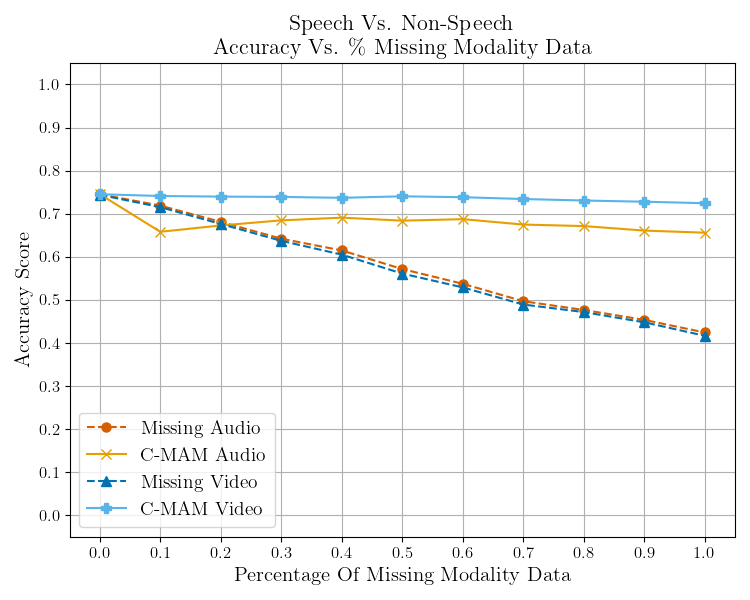
\includegraphics[width=0.9\textwidth]{imgs/sns_results/accuracy.png} % first figure itself
%     \end{minipage}\hfill
%     % Remove or comment out this line
%     \begin{minipage}{0.45\textwidth}
%         \centering
%         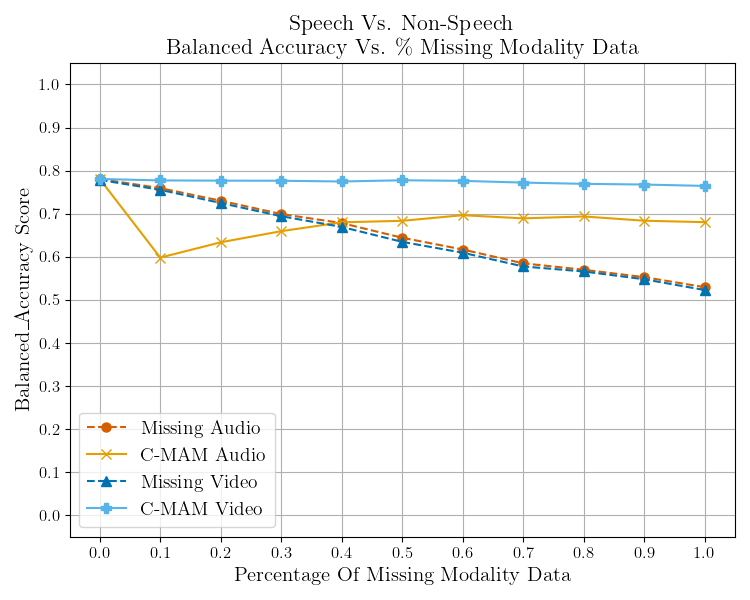
\includegraphics[width=0.9\textwidth]{imgs/sns_results/balanced_accuracy.png} % second figure itself
%     \end{minipage}
%         \begin{minipage}{0.45\textwidth}
%         \centering
%         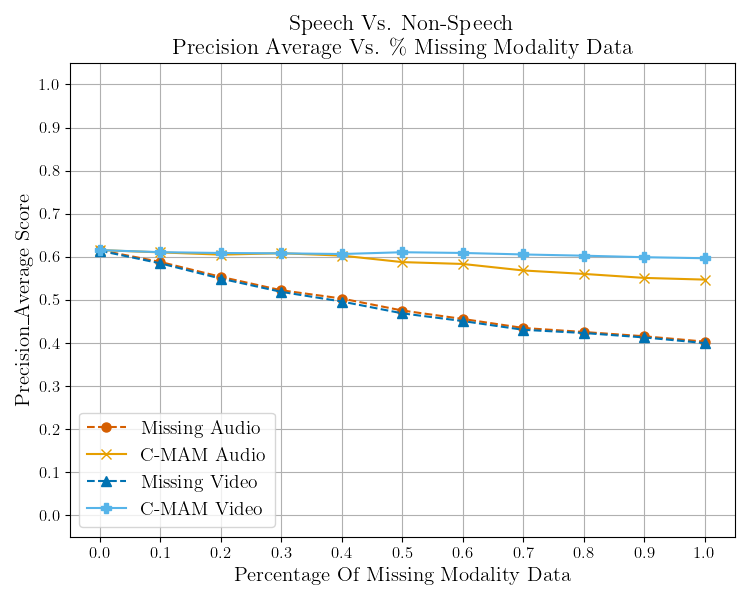
\includegraphics[width=0.9\textwidth]{imgs/sns_results/precision_average.png} % first figure itself
%     \end{minipage}\hfill
%     % Remove or comment out this line
%     \begin{minipage}{0.45\textwidth}
%         \centering
%         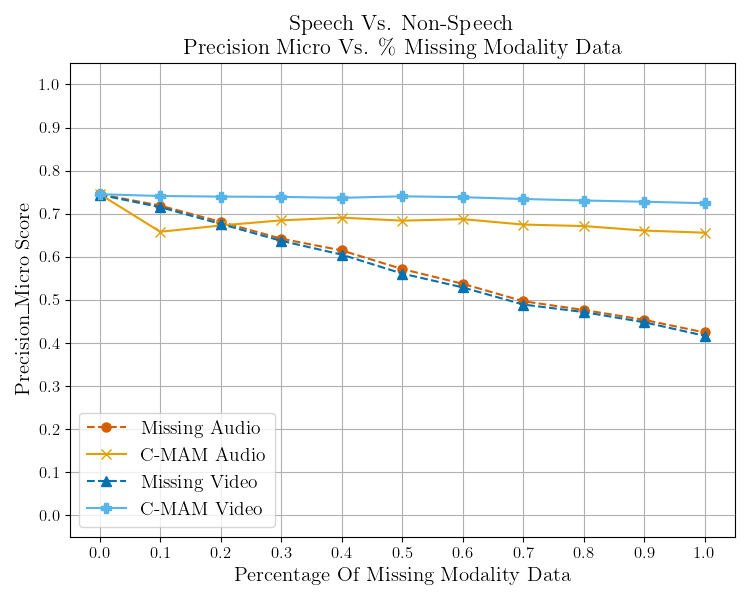
\includegraphics[width=0.9\textwidth]{imgs/sns_results/precision_micro.png} % second figure itself
%     \end{minipage}
%             \begin{minipage}{0.45\textwidth}
%         \centering
%         \includegraphics[width=0.9\textwidth]{imgs/sns_results/precision_macro.png} % first figure itself
%     \end{minipage}\hfill
%     % Remove or comment out this line
%     \begin{minipage}{0.45\textwidth}
%         \centering
%         \includegraphics[width=0.9\textwidth]{imgs/sns_results/precision_weighted.png} % second figure itself
%     \end{minipage}

%             \begin{minipage}{0.45\textwidth}
%         \centering
%         \includegraphics[width=0.9\textwidth]{imgs/sns_results/recall_average.png} % first figure itself
%     \end{minipage}\hfill
%     % Remove or comment out this line
%     \begin{minipage}{0.45\textwidth}
%         \centering
%         \includegraphics[width=0.9\textwidth]{imgs/sns_results/recall_micro.png} % second figure itself
%     \end{minipage}
% \end{figure}

% \begin{figure} \ContinuedFloat
%     \begin{minipage}{0.45\textwidth}
%         \centering
%         \includegraphics[width=0.9\textwidth]{imgs/sns_results/recall_macro.png} % first figure itself
%     \end{minipage}  
%     % Remove or comment out this line
%     \begin{minipage}{0.45\textwidth}
%         \centering
%         \includegraphics[width=0.9\textwidth]{imgs/sns_results/recall_weighted.png} % second figure itself
%     \end{minipage} 
%     \begin{minipage}{0.45\textwidth}
%         \centering
%         \includegraphics[width=0.9\textwidth]{imgs/sns_results/f1_micro.png} % second figure itself
%     \end{minipage} \hfill
%     \begin{minipage}{0.45\textwidth}
%         \centering
%         \includegraphics[width=0.9\textwidth]{imgs/sns_results/f1_macro.png} % first figure itself
%     \end{minipage} 
%     % Remove or comment out this line
%     \begin{minipage}{0.45\textwidth}
%         \centering
%         \includegraphics[width=0.9\textwidth]{imgs/sns_results/f1_weighted.png} % second figure itself
%     \end{minipage}
% \end{figure}
% \FloatBarrier
% \newpage

% Please add the following required packages to your document preamble:
% \usepackage{graphicx}
\begin{table}[h!]
\footnotesize
\centering
\caption{Hyperparameters used for the various models trained on the AVMNIST dataset.}
\label{tab:avmnist_hypparams}
\begin{tabular}{lccc}
\hline
\multicolumn{4}{c}{\textbf{AVMNIST Hyperparameters}}                     \\ \hline
\multicolumn{1}{l|}{\textbf{Parameter}} & \textbf{MM} & \textbf{C-MAM Audio} & \textbf{C-MAM Image} \\ \hline
\multicolumn{1}{l|}{\textbf{Epochs}}        & 40           & 20   & 20   \\
\multicolumn{1}{l|}{\textbf{Loss Function}} & CrossEntropy & MSE  & MSE  \\
\multicolumn{1}{l|}{\textbf{Optimizer}}     & Adam         & Adam & Adam \\
\multicolumn{1}{l|}{\textbf{Learning Rate}} & 1e-5         & 1e-3 & 1e-3 \\
\multicolumn{1}{l|}{\textbf{Weight Decay}}  & 1e-4         & 0.0  & 0.0  \\
\multicolumn{1}{l|}{\textbf{Batch Size}}    & 128          & 32   & 128  \\ \hline
\end{tabular}%
\end{table}

\begin{table}[h!]
    \footnotesize
    \caption{Architectures for each model trained on the AVMNIST dataset.}
    \label{tab:avmnist}
    \centering
    \begin{minipage}[t]{0.44\textwidth}
    \centering
    \vspace{0pt} % Align tops
        \begin{tabular}{clllllclllll}
            \hline
            \multicolumn{12}{c}{\textbf{AVMNIST Multimodal Model}}           \\ \hline
            \multicolumn{6}{c|}{\textbf{Audio Subnet}}   & \multicolumn{6}{c}{\textbf{Video Subnet}} \\ \hline
            \multicolumn{6}{c|}{}   & \multicolumn{6}{c}{ConvBlock  - (1, 32, 32, 32)} \\ \cline{7-12}
            \multicolumn{6}{c|}{}   & \multicolumn{6}{c}{MaxPool2d - (2, 2)} \\ \cline{7-12}
            \multicolumn{6}{c|}{}   & \multicolumn{6}{c}{ConvBlock - (32, 64, 64, 64)} \\ \cline{7-12}
            \multicolumn{6}{c|}{}   & \multicolumn{6}{c}{MaxPool2d - (2, 2)} \\ \hline
            \multicolumn{6}{c|}{ConvBlock  - (1, 32, 32, 32)}      & \multicolumn{6}{c}{Linear - (3136, 128)}    \\ \hline
            \multicolumn{6}{c|}{MaxPool2d - (2, 2)} &           \multicolumn{6}{c}{ReLU}      \\ \hline
            \multicolumn{6}{c|}{ConvBlock - (32, 64, 64, 64)}       & \multicolumn{6}{c}{Linear - (3136, 128)}    \\ \hline
            \multicolumn{6}{c|}{MaxPool2d - (3, 3)}     & \multicolumn{6}{c}{ReLU}      \\ \hline
            \multicolumn{6}{c|}{Linear - (4800, 128)}   & \multicolumn{6}{c}{Linear - (128, 64)}    \\ \hline
            \multicolumn{12}{c}{Linear - (128 + 64, 64)}                                      \\ \hline
            \multicolumn{12}{c}{ReLU}                                        \\ \hline
            \multicolumn{12}{c}{Linear - (64, 32)}                                      \\ \hline
            \multicolumn{12}{c}{ReLU}                                        \\ \hline
            \multicolumn{12}{c}{Linear - (32, 10)}                                      \\ \hline
        \end{tabular}
    \end{minipage}%
    \hfill
    \begin{minipage}[t]{0.19\textwidth}
    \centering
    \vspace{0pt} % Align tops
        \begin{tabular}{|clllll|}
        \hline
        \multicolumn{6}{c}{\textbf{AVMNIST Audio C-MAM}} \\ \hline
            \multicolumn{6}{c}{ConvBlock - (1, 32, 32, 32)}                     \\ \hline
            \multicolumn{6}{c}{MaxPool2d - (2, 2)}                       \\ \hline
            \multicolumn{6}{c}{ConvBlock - (32, 64, 64, 64)}                     \\ \hline
            \multicolumn{6}{c}{MaxPool2d - (2, 2)}                        \\ \hline
            \multicolumn{6}{c}{Linear - (3136, 128)}                        \\ \hline
            \multicolumn{6}{c}{ReLU}                        \\ \hline
            \multicolumn{6}{c}{Linear - (128, 64)}                        \\ \hline
            \multicolumn{6}{c}{ReLU}                        \\ \hline
            \multicolumn{6}{c}{Linear - {64, 128}}\\ \hline
        \end{tabular}
    \end{minipage}%
    \hfill
    \begin{minipage}[t]{0.2\textwidth}
    \centering
    \vspace{0pt} % Align tops
        \begin{tabular}{|clllll|}
        \hline
        \multicolumn{6}{c}{\textbf{AVMNIST Image C-MAM}} \\ \hline
        \multicolumn{6}{c}{ConvBlock - (1, 32, 32, 32)}                     \\ \hline
        \multicolumn{6}{c}{MaxPool2d - (2, 2)}                       \\ \hline
        \multicolumn{6}{c}{ConvBlock - (32, 64, 64, 64)}                     \\ \hline
        \multicolumn{6}{c}{MaxPool2d - (3, 3)}                        \\ \hline
        \multicolumn{6}{c}{Linear - (4800, 128)}                   \\ \hline
        \multicolumn{6}{c}{ReLU}                   \\ \hline
        \multicolumn{6}{c}{Linear - (128, 64)}                   \\ \hline
        \end{tabular}
    \end{minipage}%
    \hfill
\end{table}


% Please add the following required packages to your document preamble:
% \usepackage{graphicx}
\begin{table}[h!]
\footnotesize
\centering
\caption{Hyperparameters used for the various models trained on the Kinetics-Sounds dataset.}
\label{tab:ks_hypparams}
\begin{tabular}{lccc}
\hline
\multicolumn{4}{c}{\textbf{Kinetics-Sounds Hyperparameters}}             \\ \hline
\multicolumn{1}{l|}{\textbf{Parameter}} & \textbf{MM} & \textbf{C-MAM Audio} & \textbf{C-MAM Video} \\ \hline
\multicolumn{1}{l|}{\textbf{Epochs}}        & 60           & 50   & 60   \\
\multicolumn{1}{l|}{\textbf{Loss Function}} & CrossEntropy & MSE  & MSE  \\
\multicolumn{1}{l|}{\textbf{Optimizer}}     & Adam         & Adam & Adam \\
\multicolumn{1}{l|}{\textbf{Learning Rate}} & 5e-4         & 1e-3 & 1e-3 \\
\multicolumn{1}{l|}{\textbf{Weight Decay}}  & 4e-5         & 4e-5 & 4e-5 \\
\multicolumn{1}{l|}{\textbf{Batch Size}}    & 128          & 32   & 128  \\ \hline
\end{tabular}%
\end{table}
\begin{table}[h!]
\footnotesize
    \caption{Architectures for each model trained on the Kinetics-Sounds dataset.}    \centering
    \begin{minipage}[t]{0.44\textwidth}
    \centering
    \vspace{0pt} % Align tops
    \begin{tabular}{clllllclllll}
        \hline
        \multicolumn{12}{c}{\textbf{Kinetics-Sounds Multimodal Model}}                                   \\ \hline
        \multicolumn{6}{c|}{\textbf{Audio Subnet}}           & \multicolumn{6}{c}{\textbf{Video Subnet}} \\ \hline
        \multicolumn{6}{c|}{ConvBlock - (1, 32, 32, 64)}     & \multicolumn{6}{c}{\multirow{9}{*}{}}     \\ \cline{1-6}
        \multicolumn{6}{c|}{Dropout - (0.55)}                & \multicolumn{6}{c}{}                      \\ \cline{1-6}
        \multicolumn{6}{c|}{AvgPool2d - (2, 2)}              & \multicolumn{6}{c}{}                      \\ \cline{1-6}
        \multicolumn{6}{c|}{ConvBlock - (64, 64, 64, 64)}    & \multicolumn{6}{c}{}                      \\ \cline{1-6}
        \multicolumn{6}{c|}{Dropout - (0.33)}                & \multicolumn{6}{c}{}                      \\ \cline{1-6}
        \multicolumn{6}{c|}{AvgPool2d - (4, 4)}              & \multicolumn{6}{c}{}                      \\ \cline{1-6}
        \multicolumn{6}{c|}{ConvBlock - (64, 128, 128, 128)} & \multicolumn{6}{c}{}                      \\ \cline{1-6}
        \multicolumn{6}{c|}{Dropout - (0.33)}                & \multicolumn{6}{c}{}                      \\ \cline{1-6}
        \multicolumn{6}{c|}{AvgPool2d - (4, 8)}              & \multicolumn{6}{c}{}                      \\ \hline
        \multicolumn{6}{c|}{Linear - (512, 64)}              & \multicolumn{6}{c}{Linear - (400, 256)}   \\ \hline
        \multicolumn{6}{c|}{ReLU}                            & \multicolumn{6}{c}{ReLU}                  \\ \hline
        \multicolumn{6}{c|}{Dropout - (0.55)}                & \multicolumn{6}{c}{Dropout - (0.55)}      \\ \hline
        \multicolumn{6}{c|}{Linear - (64, 32)}               & \multicolumn{6}{c}{Linear - (256, 128)}   \\ \hline
        \multicolumn{12}{c}{Linear - (32 + 128, 64)}                                                     \\ \hline
        \multicolumn{12}{c}{ReLU}                                                                        \\ \hline
        \multicolumn{12}{c}{Dropout - (0.4)}                                                             \\ \hline
        \multicolumn{12}{c}{Linear - (64, 32)}                                                           \\ \hline
        \multicolumn{12}{c}{ReLU}                                                                        \\ \hline
        \multicolumn{12}{c}{Dropout - (0.4)}                                                             \\ \hline
        \multicolumn{12}{c}{Linear - (32, 26)}                                                           \\ \hline
    \end{tabular}
    \end{minipage}%
    \hfill
    \begin{minipage}[t]{0.30\textwidth}
    \centering
    \vspace{0pt} % Align tops
    \begin{tabular}{|clllll|}
        \hline
        \multicolumn{6}{c}{\textbf{Kinetics-Sounds Audio C-MAM}} \\ \hline
        \multicolumn{6}{c}{Linear - (400, 256)} \\ \hline
        \multicolumn{6}{c}{ReLU}                \\ \hline
        \multicolumn{6}{c}{Dropout - (0.55)}    \\ \hline
        \multicolumn{6}{c}{Linear - (256, 128)} \\ \hline
        \multicolumn{6}{c}{ReLU} \\ \hline
        \multicolumn{6}{c}{Linear - (128, 128)} \\ \hline
        \multicolumn{6}{c}{BatchNorm1d - (128)} \\ \hline
        \multicolumn{6}{c}{Dropout - (0.4)} \\ \hline
        \multicolumn{6}{c}{ReLU} \\ \hline
        \multicolumn{6}{c}{Linear - (128, 64)} \\ \hline
        \multicolumn{6}{c}{BatchNorm1d - (64)} \\ \hline
        \multicolumn{6}{c}{Dropout - (0.2)} \\ \hline
        \multicolumn{6}{c}{Linear - (64, 32)} \\ \hline
        \end{tabular}
    \end{minipage}%
    \hfill
    \centering
    \begin{minipage}[t]{0.2\textwidth}
    \centering
    \vspace{0pt} % Align tops
        \begin{tabular}{|clllll|}
        \hline
        \multicolumn{6}{c}{\textbf{Kinetics-Sounds Video C-MAM}} \\ \hline
        \multicolumn{6}{c}{ConvBlock - (1, 32, 32, 64)}    \\ \hline
        \multicolumn{6}{c}{Dropout - (0.55)}                \\ \hline
        \multicolumn{6}{c}{AvgPool2d - (2, 2)}              \\ \hline
        \multicolumn{6}{c}{ConvBlock - (64, 64, 64, 64)}    \\ \hline
        \multicolumn{6}{c}{Dropout - (0.33)}                \\ \hline
        \multicolumn{6}{c}{AvgPool2d - (4, 4)}              \\ \hline
        \multicolumn{6}{c}{ConvBlock - (64, 128, 128, 128)} \\ \hline
        \multicolumn{6}{c}{Dropout - (0.33)}                \\ \hline
        \multicolumn{6}{c}{AvgPool2d - (4, 8)}              \\ \hline
        \multicolumn{6}{c}{Linear - (512, 64)}              \\ \hline
        \multicolumn{6}{c}{ReLU}                            \\ \hline
        \multicolumn{6}{c}{Dropout - (0.55)}                \\ \hline
        \multicolumn{6}{c}{Linear - (64, 32)}               \\ \hline
        \multicolumn{6}{c}{ReLU}               \\ \hline
        \multicolumn{6}{c}{Linear - (32, 64)}               \\ \hline
        \multicolumn{6}{c}{BatchNorm1d - (64)}               \\ \hline
        \multicolumn{6}{c}{ReLU}               \\ \hline
        \multicolumn{6}{c}{Linear - (64, 128)}               \\ \hline
        \end{tabular}
    \end{minipage}%
    \hfill
\end{table}


% Please add the following required packages to your document preamble:
% \usepackage{graphicx}
\begin{table}[h!]
\footnotesize

\centering
\caption{Hyperparameters used for the various models trained on the MM-IMDb dataset.}
\label{tab:mmimdb_hypparams}
\begin{tabular}{lccc}
\hline
\multicolumn{4}{c}{\textbf{MM-IMDb Hyperparameters}}             \\ \hline
\multicolumn{1}{l|}{\textbf{Parameter}}     & \textbf{MM}        & \textbf{C-MAM Image} & \textbf{C-MAM Text} \\ \hline
\multicolumn{1}{l|}{\textbf{Epochs}}        & 200  & 200  & 200  \\
\multicolumn{1}{l|}{\textbf{Loss Function}} & BinaryCrossEntropy & MSE                  & MSE                 \\
\multicolumn{1}{l|}{\textbf{Optimizer}}     & Adam & Adam & Adam \\
\multicolumn{1}{l|}{\textbf{Learning Rate}} & 1e-5 & 1e-5 & 1e-5 \\
\multicolumn{1}{l|}{\textbf{Weight Decay}}  & 1e-3 & 1e-3 & 1e-3 \\
\multicolumn{1}{l|}{\textbf{Batch Size}}    & 128  & 128  & 128  \\ \hline
\end{tabular}%
\end{table}

\begin{table}[h!]
    \footnotesize
    \caption{Maxout layer used in the various MM-IMDb models trained.}
    \label{tab:maxout}
    \begin{tabular}{ll}
    \hline
    \multicolumn{2}{c}{\textbf{MaxOut - (input\_dim, output\_dim, N\_LAYERS)}}                             \\ \hline
    \multicolumn{1}{c|}{\multirow{2}{*}{\textbf{MAX}}} & Linear$_1$ - (input\_dim, output\_dim)           \\ \cline{2-2} 
    \multicolumn{1}{c|}{}                              & Linear$_{N\_LAYERS}$ - (input\_dim,output\_dim) \\ \hline
    \end{tabular}
\end{table}

\begin{table}[h!]
\footnotesize
    \caption{Architectures for each model trained on the MM-IMDb dataset.}    \centering
    \begin{minipage}[t]{0.49\textwidth}
    \centering
    \vspace{0pt} % Align tops
    \begin{tabular}{clllllclllll}
        \hline
        \multicolumn{12}{c}{\textbf{MM-IMDb Multimodal Model}}                                \\ \hline
        \multicolumn{6}{c|}{\textbf{Image Subnet}} & \multicolumn{6}{c}{\textbf{Text Subnet}} \\ \hline
        \multicolumn{6}{c|}{BatchNorm1d - (4096)}  & \multicolumn{6}{c}{BatchNorm1d - (300)}  \\ \hline
        \multicolumn{6}{c|}{Linear - (4096, 512)}  & \multicolumn{6}{c}{Linear - (300, 512)}  \\ \hline
        \multicolumn{6}{c|}{TanH}                  & \multicolumn{6}{c}{TanH}                 \\ \hline
        \multicolumn{12}{c}{Linear - (512 + 512, 1)}                                          \\ \hline
        \multicolumn{12}{c}{Sigmoid}                                                          \\ \hline
        \multicolumn{12}{c}{BatchNorm1d - (512)}                                              \\ \hline
        \multicolumn{12}{c}{Maxout - (512, 512)}                                              \\ \hline
        \multicolumn{12}{c}{Dropout}                                                  \\ \hline
        \multicolumn{12}{c}{BatchNorm1d - (512)}                                              \\ \hline
        \multicolumn{12}{c}{Maxout - (512, 512)}                                              \\ \hline
        \multicolumn{12}{c}{Dropout}                                                  \\ \hline
        \multicolumn{12}{c}{BatchNorm1d - (512)}                                              \\ \hline
        \multicolumn{12}{c}{Linear - (512, 23)}                                               \\ \hline
        \end{tabular}%

    \end{minipage}%
    \hfill
    \begin{minipage}[t]{0.2\textwidth}
    \centering
    \vspace{0pt} % Align tops
    \begin{tabular}{clllll}
        \hline
        \multicolumn{6}{c}{\textbf{MM-IMDb Text C-MAM}} \\ \hline
        \multicolumn{6}{c}{Linear - (300, 512)}         \\ \hline
        \multicolumn{6}{c}{BatchNorm1d - (512)}         \\ \hline
        \multicolumn{6}{c}{Linear - (512, 256)}         \\ \hline
        \multicolumn{6}{c}{Dropout}                     \\ \hline
        \multicolumn{6}{c}{Linear - (256, 512)}         \\ \hline
        \end{tabular}%
    \end{minipage}%
    \hfill
    \begin{minipage}[t]{0.2\textwidth}
    \centering
    \vspace{0pt} % Align tops
    \begin{tabular}{clllll}
        \hline
        \multicolumn{6}{c}{\textbf{MM-IMDb Image C-MAM}} \\ \hline
        \multicolumn{6}{c}{Linear - (4096, 512)}         \\ \hline
        \multicolumn{6}{c}{BatchNorm1d - (512)}          \\ \hline
        \multicolumn{6}{c}{ReLU}                         \\ \hline
        \multicolumn{6}{c}{Dropout}                      \\ \hline
        \multicolumn{6}{c}{Linear - (512, 256)}          \\ \hline
        \multicolumn{6}{c}{BatchNorm1d - (256)}          \\ \hline
        \multicolumn{6}{c}{ReLU}                         \\ \hline
        \multicolumn{6}{c}{Dropout}                      \\ \hline
        \multicolumn{6}{c}{Linear - (256, 512)}          \\ \hline
        \end{tabular}%
    \end{minipage}%
    \hfill
\end{table}




